\section{Cross-section Ratio, \texorpdfstring{\ratio}{R-32)}}
\label{sec:cross_section}

\begin{table}[!htbp]
 \caption{Differential cross-sections ($\times$ 10$^{-3}$(pb/GeV)) and the cross-section ratio \ratio at detector level in each bin of \httwo, along with statistical uncertainty (in \%).}
 \label{tab:ratio_32}
 \centering
 \vspace{2mm}
 %\begin{tabular}{cccccccc} \hline \hline
 \hspace*{-4mm}\begin{tabular}{>{\centering\arraybackslash}m{0.81in}>{\centering\arraybackslash}m{1.03in}>{\centering\arraybackslash}m{0.48in}>{\centering\arraybackslash}m{1.03in}>{\centering\arraybackslash}m{0.48in}>{\centering\arraybackslash}m{0.5in}>{\centering\arraybackslash}m{0.48in}} \hline \hline
      & {\bf 2-jet } & {\bf Stat.} & {\bf 3-jet } & {\bf Stat.} & {\bf Ratio} & {\bf Stat.} \rbtrrn \\
 {\bf Bin} & {\bf cross-section} & {\bf unc.} & {\bf cross-section} & {\bf unc.} & {\bf \ratio} & {\bf unc.} \rbtrrn \\ \hline 
300 - 330 & 29772.726 & 0.211 & 2640.629 & 0.707 & 0.089 & $^{+0.665}_{-0.661}$ \rbtrrn \\ \hline
330 - 360 & 16792.917 & 0.231 & 1773.485 & 0.704 & 0.106 & $^{+0.523}_{-0.521}$ \rbtrrn \\ \hline
360 - 390 & 9889.326 & 0.182 & 1176.544 & 0.526 & 0.119 & $^{+0.485}_{-0.483}$ \rbtrrn \\ \hline
390 - 420 & 5976.777 & 0.179 & 778.034 & 0.492 & 0.130 & $^{+0.206}_{-0.206}$ \rbtrrn \\ \hline
420 - 450 & 3731.760 & 0.067 & 522.624 & 0.180 & 0.140 & $^{+0.167}_{-0.167}$ \rbtrrn \\ \hline
450 - 480 & 2398.741 & 0.084 & 357.622 & 0.217 & 0.149 & $^{+0.201}_{-0.200}$ \rbtrrn \\ \hline
480 - 510 & 1570.192 & 0.104 & 246.051 & 0.262 & 0.157 & $^{+0.241}_{-0.241}$ \rbtrrn \\ \hline
510 - 540 & 1048.665 & 0.127 & 171.080 & 0.314 & 0.163 & $^{+0.288}_{-0.287}$ \rbtrrn \\ \hline
540 - 570 & 713.042 & 0.154 & 119.566 & 0.376 & 0.168 & $^{+0.344}_{-0.343}$ \rbtrrn \\ \hline
570 - 600 & 490.776 & 0.186 & 84.798 & 0.447 & 0.173 & $^{+0.407}_{-0.406}$ \rbtrrn \\ \hline
600 - 640 & 325.046 & 0.198 & 57.463 & 0.470 & 0.177 & $^{+0.427}_{-0.426}$ \rbtrrn \\ \hline
640 - 680 & 205.727 & 0.248 & 37.282 & 0.583 & 0.181 & $^{+0.529}_{-0.527}$ \rbtrrn \\ \hline
680 - 720 & 133.674 & 0.308 & 24.859 & 0.714 & 0.186 & $^{+0.646}_{-0.643}$ \rbtrrn \\ \hline
720 - 760 & 87.911 & 0.380 & 16.560 & 0.875 & 0.188 & $^{+0.791}_{-0.786}$ \rbtrrn \\ \hline
760 - 800 & 58.657 & 0.465 & 11.056 & 1.071 & 0.188 & $^{+0.968}_{-0.961}$ \rbtrrn \\ \hline
800 - 850 & 38.106 & 0.516 & 7.318 & 1.178 & 0.192 & $^{+1.063}_{-1.054}$ \rbtrrn \\ \hline
850 - 900 & 23.587 & 0.656 & 4.600 & 1.485 & 0.195 & $^{+1.339}_{-1.326}$ \rbtrrn \\ \hline
900 - 950 & 15.130 & 0.819 & 2.896 & 1.872 & 0.191 & $^{+1.694}_{-1.672}$ \rbtrrn \\ \hline
950 - 1000 & 9.696 & 1.023 & 1.812 & 2.366 & 0.187 & $^{+2.151}_{-2.116}$ \rbtrrn \\ \hline
1000 - 1060 & 6.026 & 1.185 & 1.186 & 2.670 & 0.197 & $^{+2.414}_{-2.371}$ \rbtrrn \\ \hline
1060 - 1120 & 3.668 & 1.518 & 0.716 & 3.436 & 0.195 & $^{+3.118}_{-3.046}$ \rbtrrn \\ \hline
1120 - 1180 & 2.327 & 1.906 & 0.437 & 4.398 & 0.188 & $^{+4.024}_{-3.903}$ \rbtrrn \\ \hline
1180 - 1250 & 1.419 & 2.260 & 0.265 & 5.227 & 0.187 & $^{+4.798}_{-4.627}$ \rbtrrn \\ \hline
1250 - 1320 & 0.853 & 2.915 & 0.165 & 6.623 & 0.194 & $^{+6.080}_{-5.811}$ \rbtrrn \\ \hline
1320 - 1390 & 0.477 & 3.898 & 0.080 & 9.492 & 0.169 & $^{+8.951}_{-8.355}$ \rbtrrn \\ \hline
1390 - 1460 & 0.263 & 5.249 & 0.042 & 13.131 & 0.160 & $^{+12.619}_{-11.449}$ \rbtrrn \\ \hline
1460 - 1530 & 0.192 & 6.143 & 0.029 & 15.811 & 0.151 & $^{+15.437}_{-13.698}$ \rbtrrn \\ \hline
1530 - 1600 & 0.104 & 8.362 & 0.021 & 18.570 & 0.203 & $^{+17.571}_{-15.536}$ \rbtrrn \\ \hline
1600 - 1680 & 0.060 & 10.314 & 0.009 & 26.726 & 0.149 & $^{+27.132}_{-22.170}$ \rbtrrn \\ \hline
 \hline
 \end{tabular}
\end{table}
\section{Individual Sources of Jet Energy Correction Uncertainties}
\label{sec:JECs}
{\fontsize{12pt}{12pt}\selectfont The sources of JEC considered in the current measurements are : AbsoluteStat, AbsoluteScale, AbsoluteFlavMap, AbsoluteMPFBias, Fragmentation, SinglePionECAL, SinglePionHCAL, FlavorQCD, RelativeJEREC1, RelativeJEREC2, RelativeJERHF, RelativePtBB, RelativePtEC1, RelativePtEC2, RelativePtHF, RelativeFSR, RelativeStatFSR, RelativeStatEC2, RelativeStatHF, PileUpDataMC, PileUpPtRef, PileUpPtBB, PileUpPtEC1, PileUpPtEC2 and PileUpPtHF. The AbsoluteFlavMap uncertainty is exactly zero for the 8 TeV and can be ignored. For the four sources : RelativeJERHF, RelativePtHF, RelativeStatHF, PileUpPtHF, the JEC uncertainty is exactly zero because of $|y|$ \ls 2.5 cut used in the analysis. So only 20 sources contribute to the total JEC uncertainty.} 

\begin{figure}[!hbtp]
%\begin{center}
\hspace*{-5mm}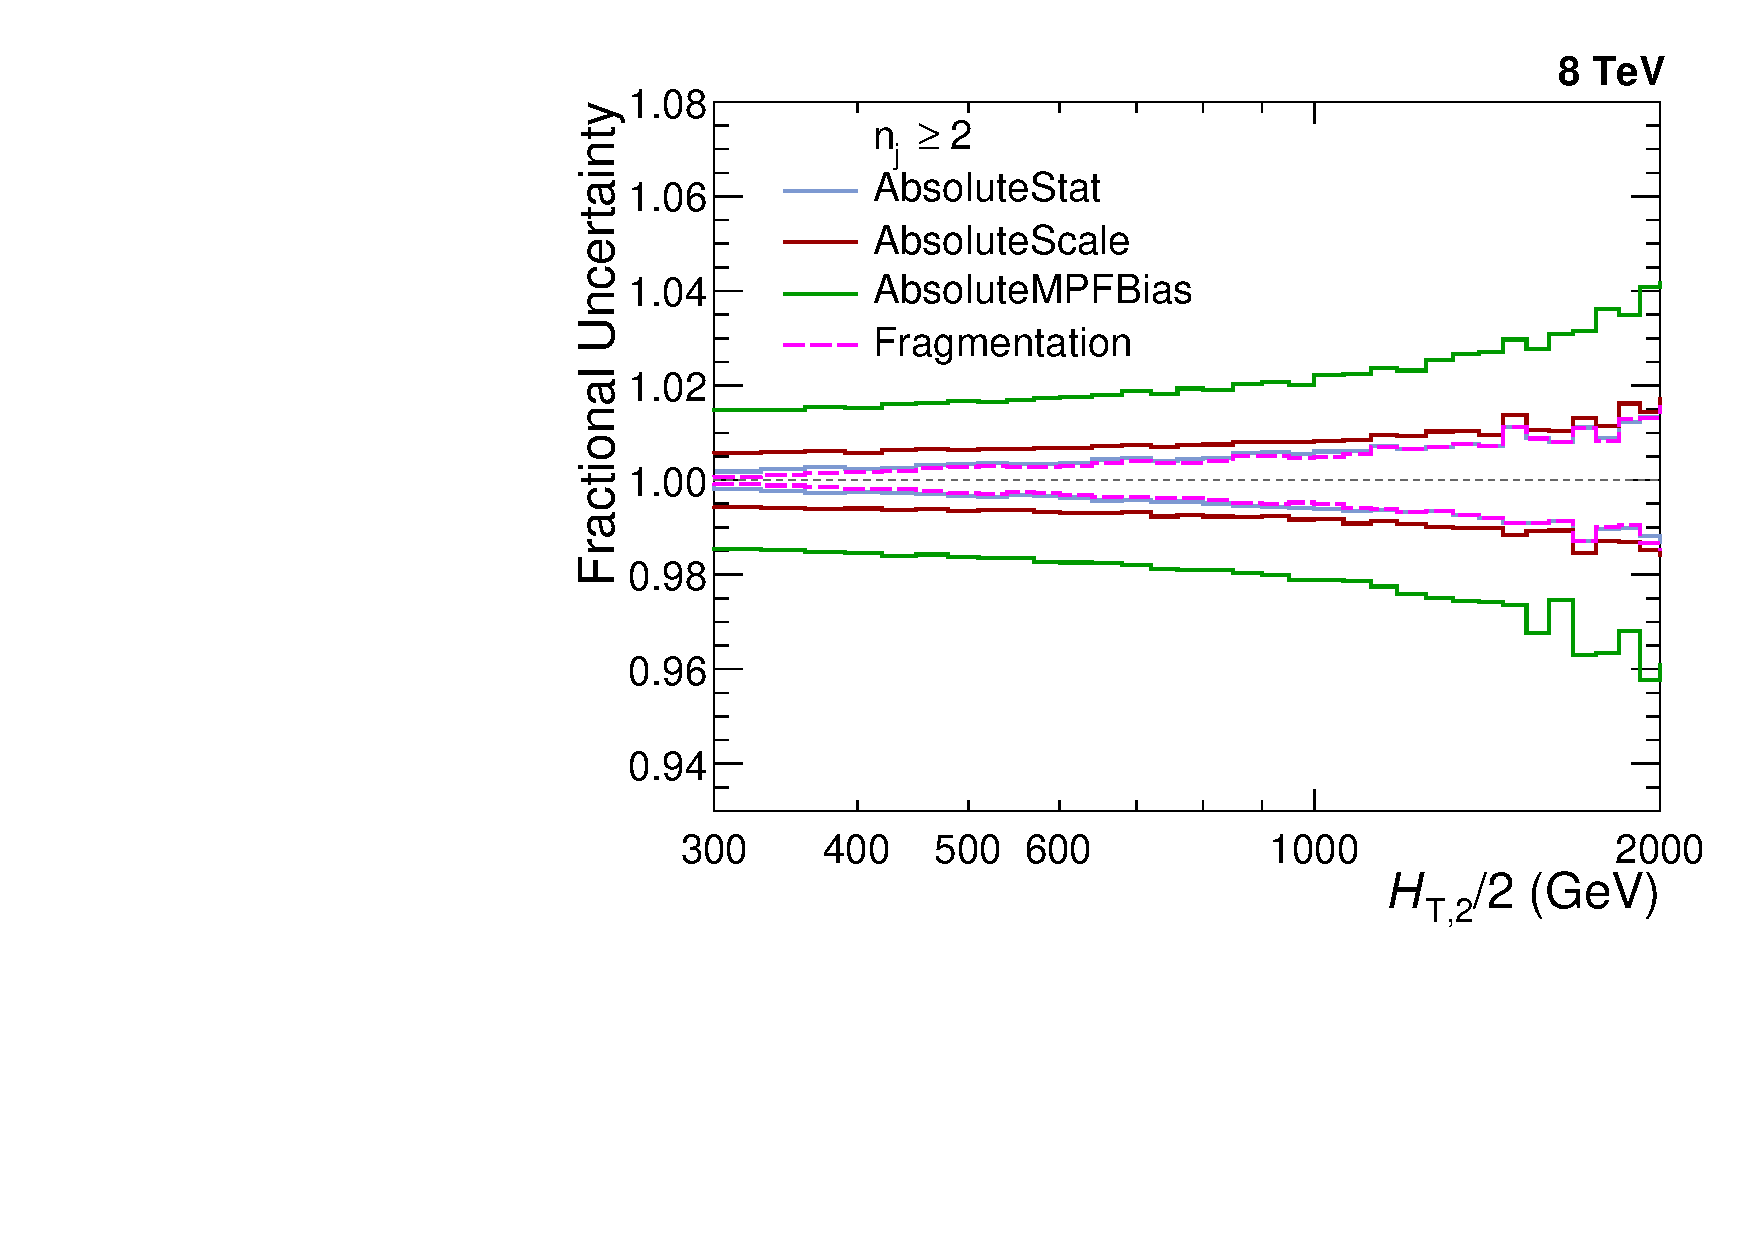
\includegraphics[width=0.51\textwidth]{/home/anter/Desktop/Thesis/Plots_HT_2_150/Single/MC_Macro_Plot_All_2_HT_2_Unc_Abs_1.pdf}%
~~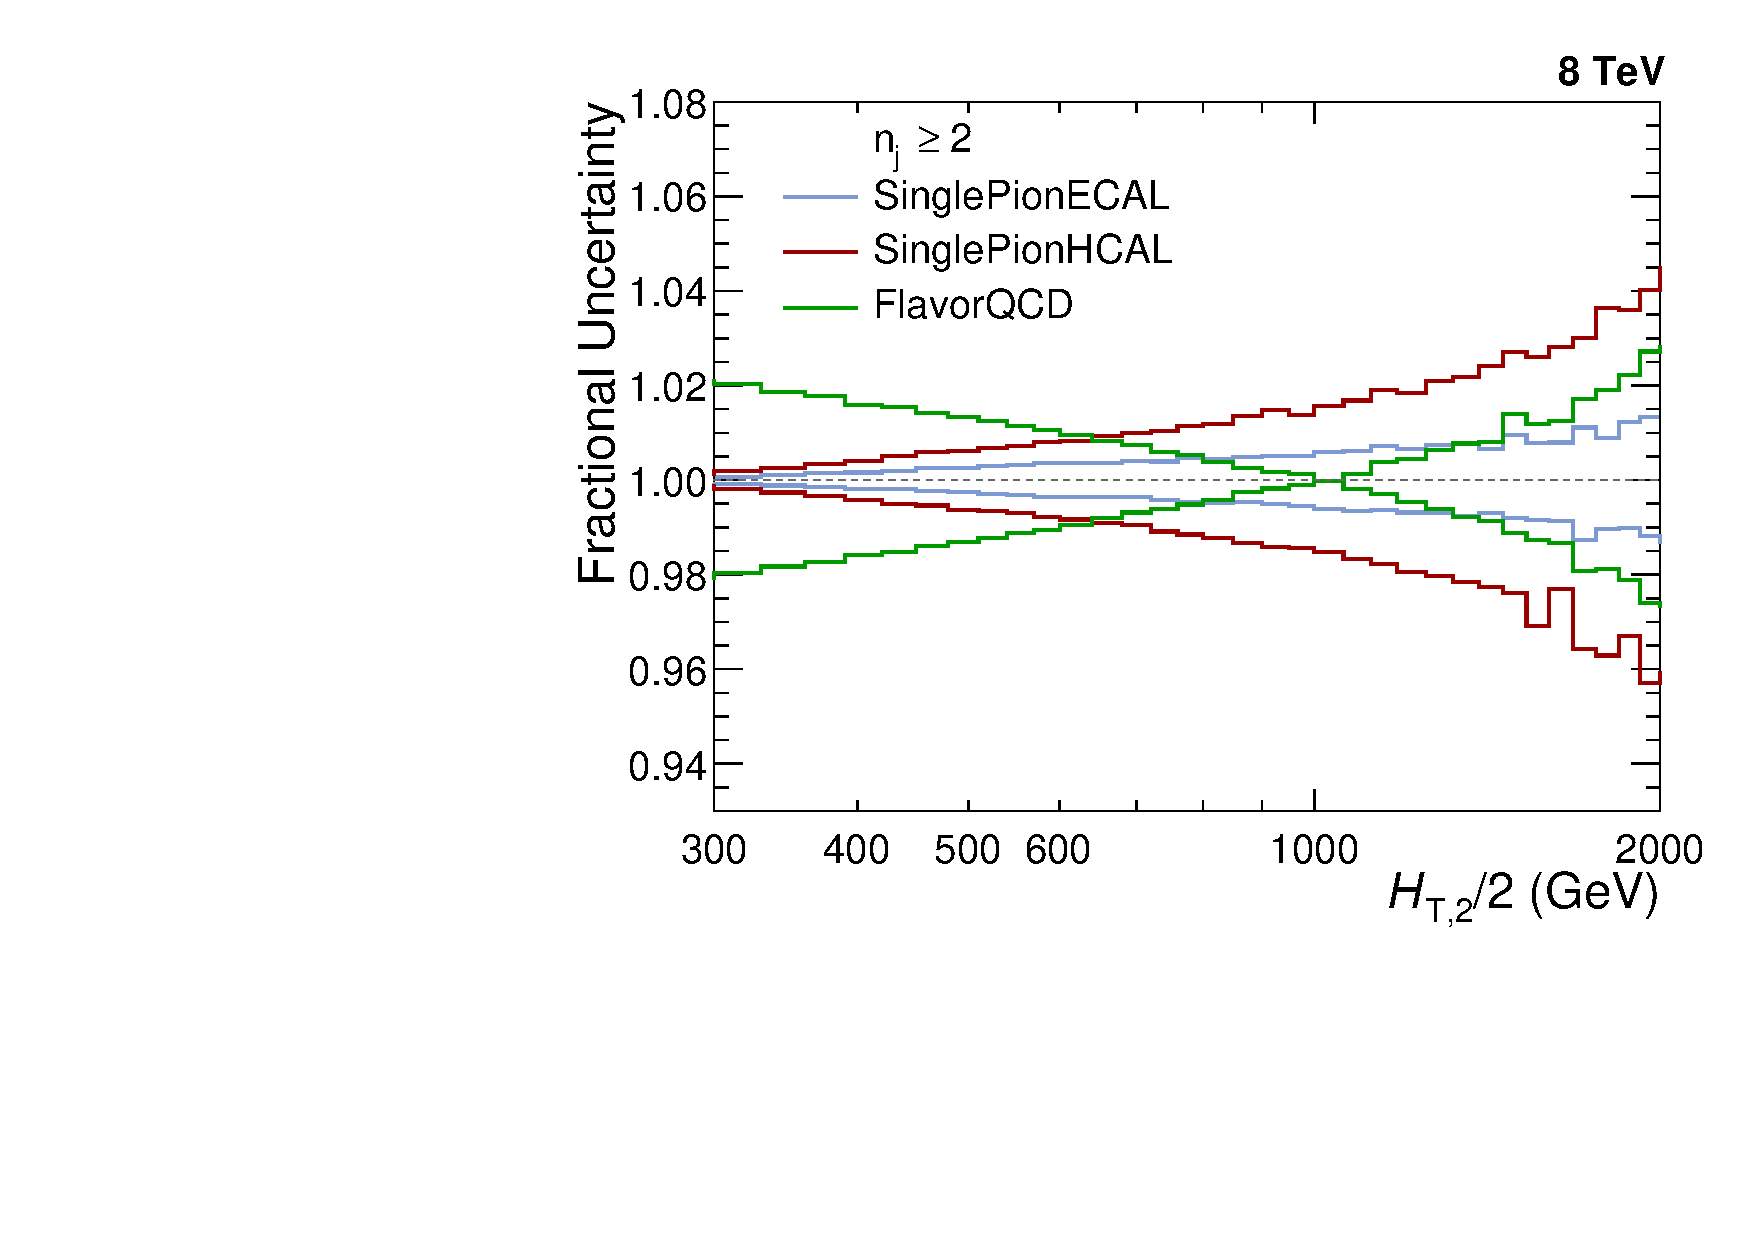
\includegraphics[width=0.51\textwidth]{/home/anter/Desktop/Thesis/Plots_HT_2_150/Single/MC_Macro_Plot_All_2_HT_2_Unc_Single_1.pdf}\\
\hspace*{-5mm}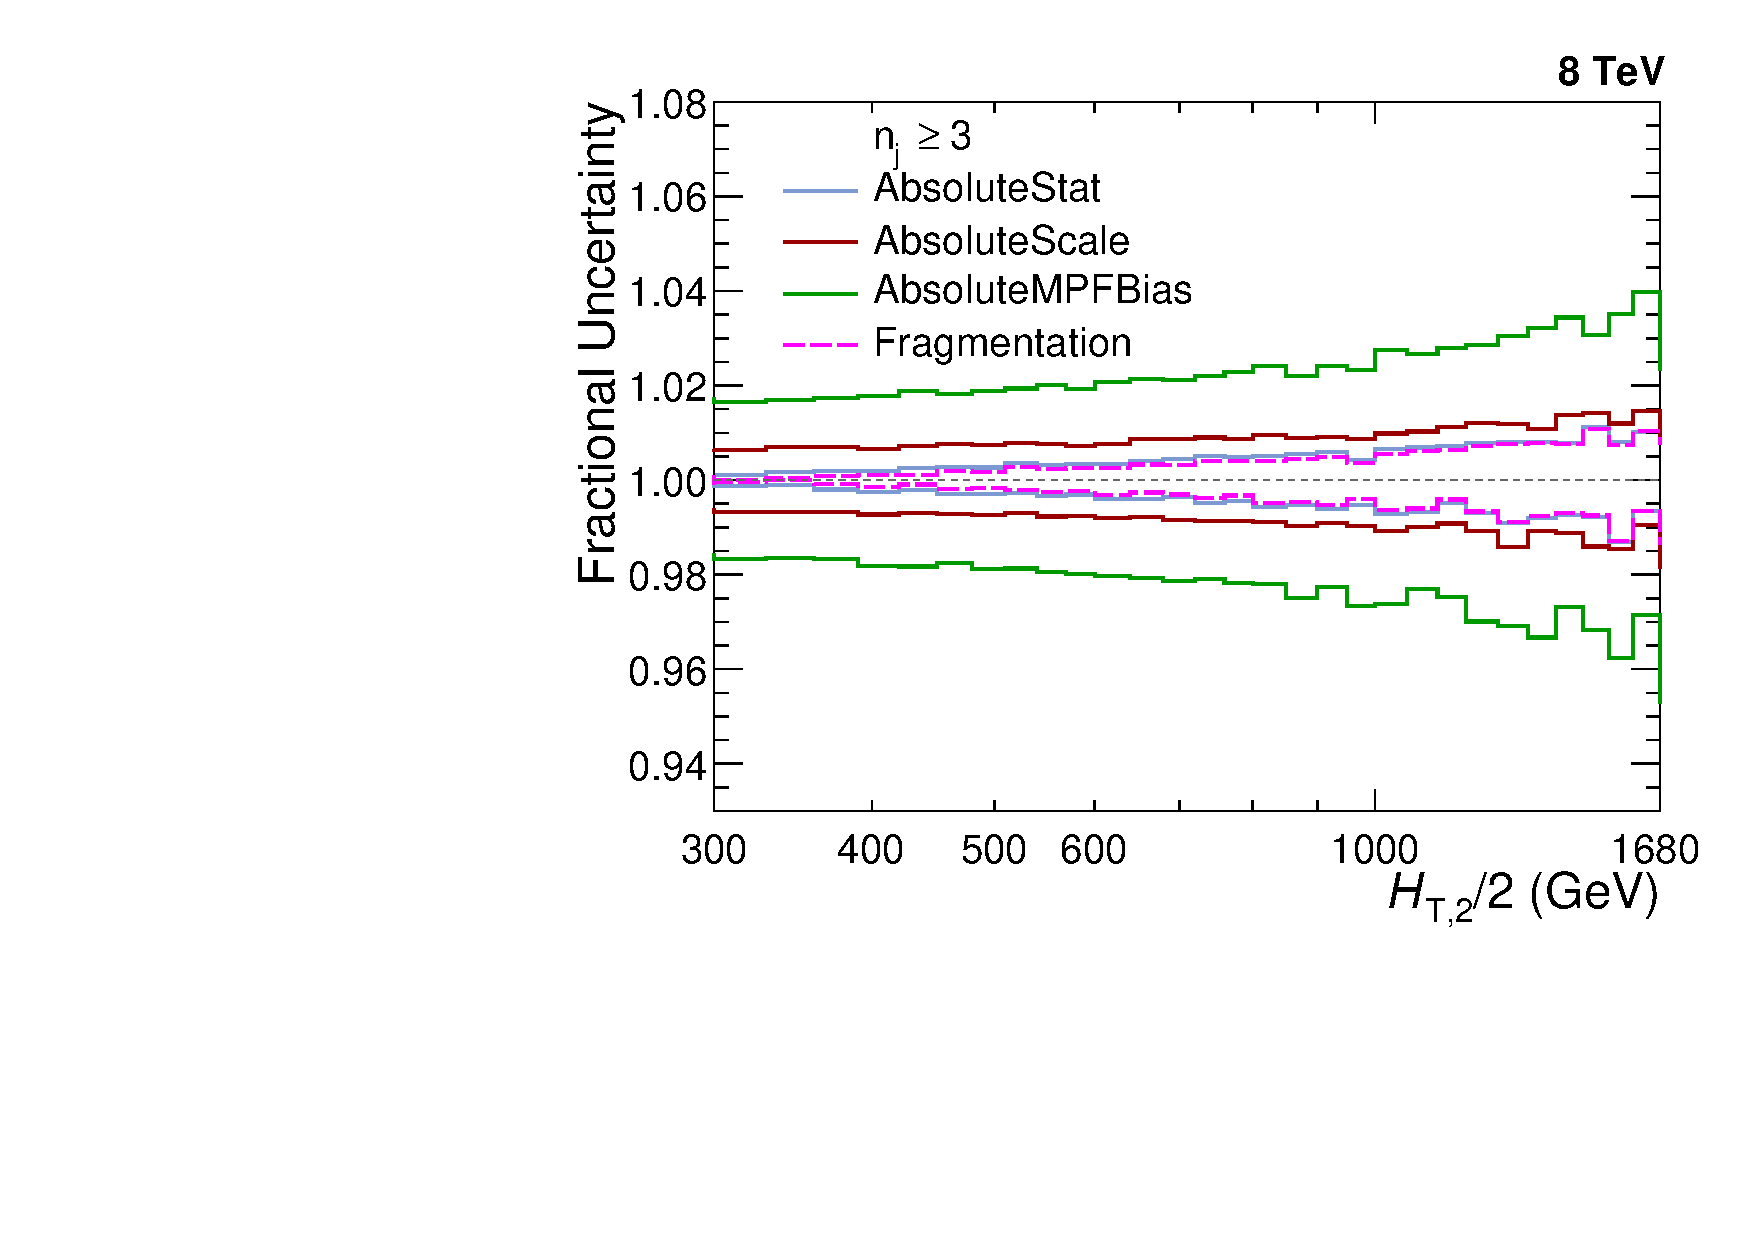
\includegraphics[width=0.51\textwidth]{/home/anter/Desktop/Thesis/Plots_HT_2_150/Single/MC_Macro_Plot_All_3_HT_2_Unc_Abs_1.pdf}%
~~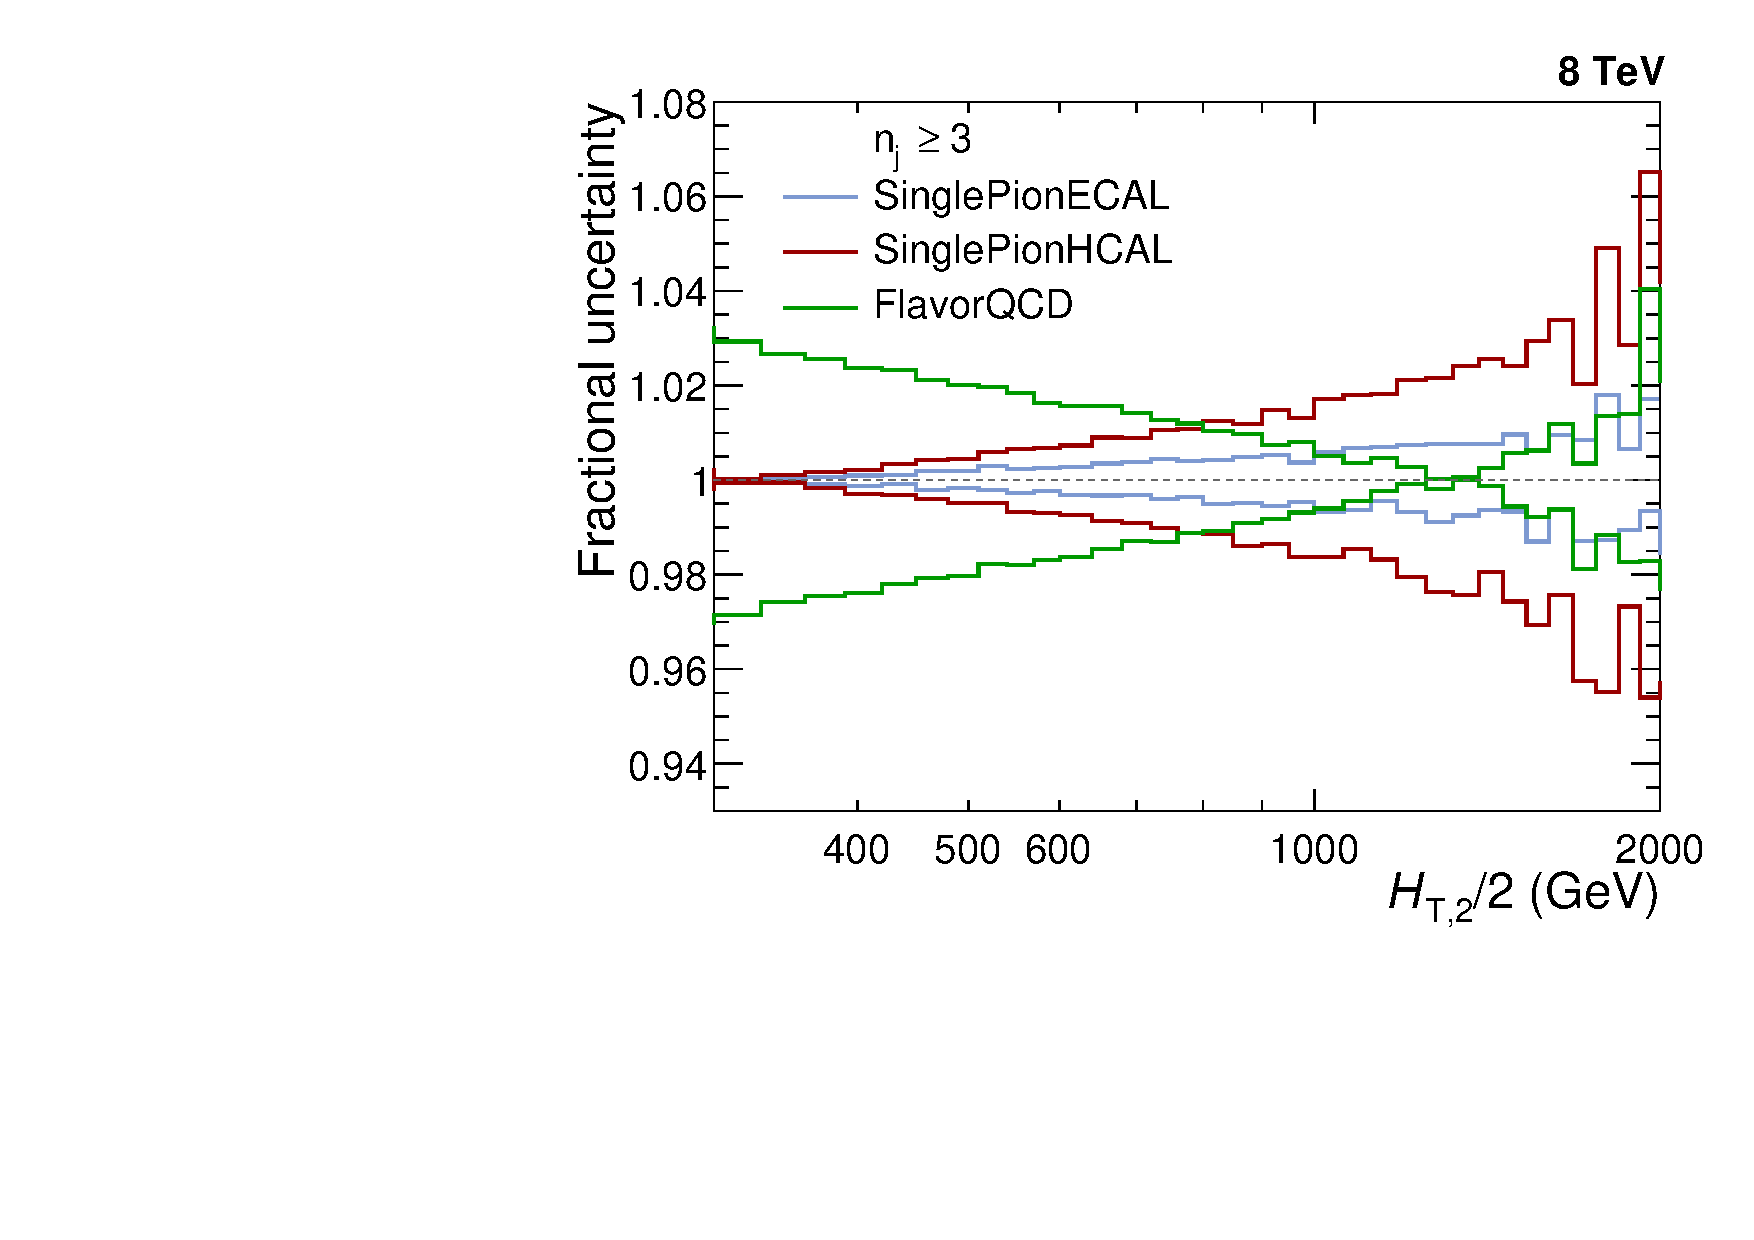
\includegraphics[width=0.51\textwidth]{/home/anter/Desktop/Thesis/Plots_HT_2_150/Single/MC_Macro_Plot_All_3_HT_2_Unc_Single_1.pdf}\\
\hspace*{-5mm}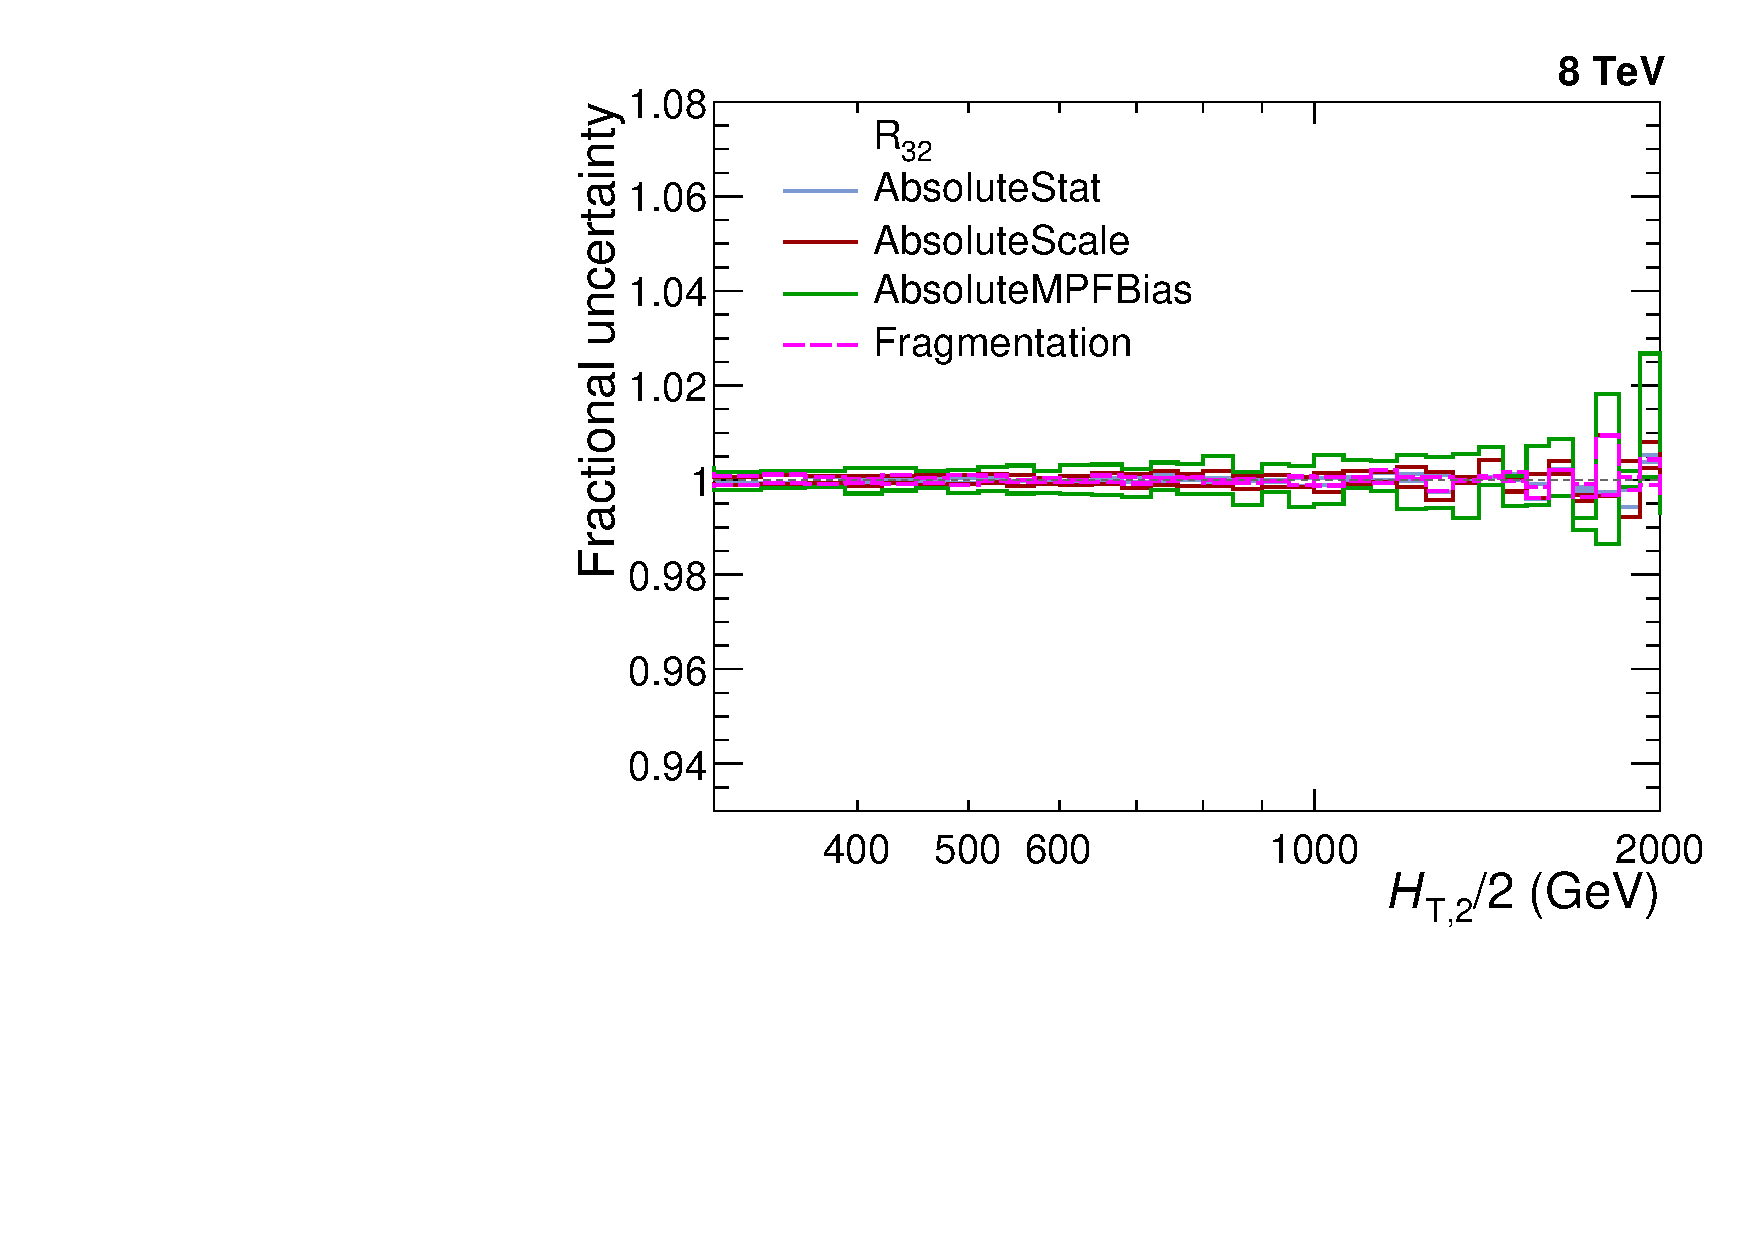
\includegraphics[width=0.51\textwidth]{/home/anter/Desktop/Thesis/Plots_HT_2_150/Single/MC_Macro_Plot_Ratio_32_HT_2_Unc_Abs_1.pdf}%
~~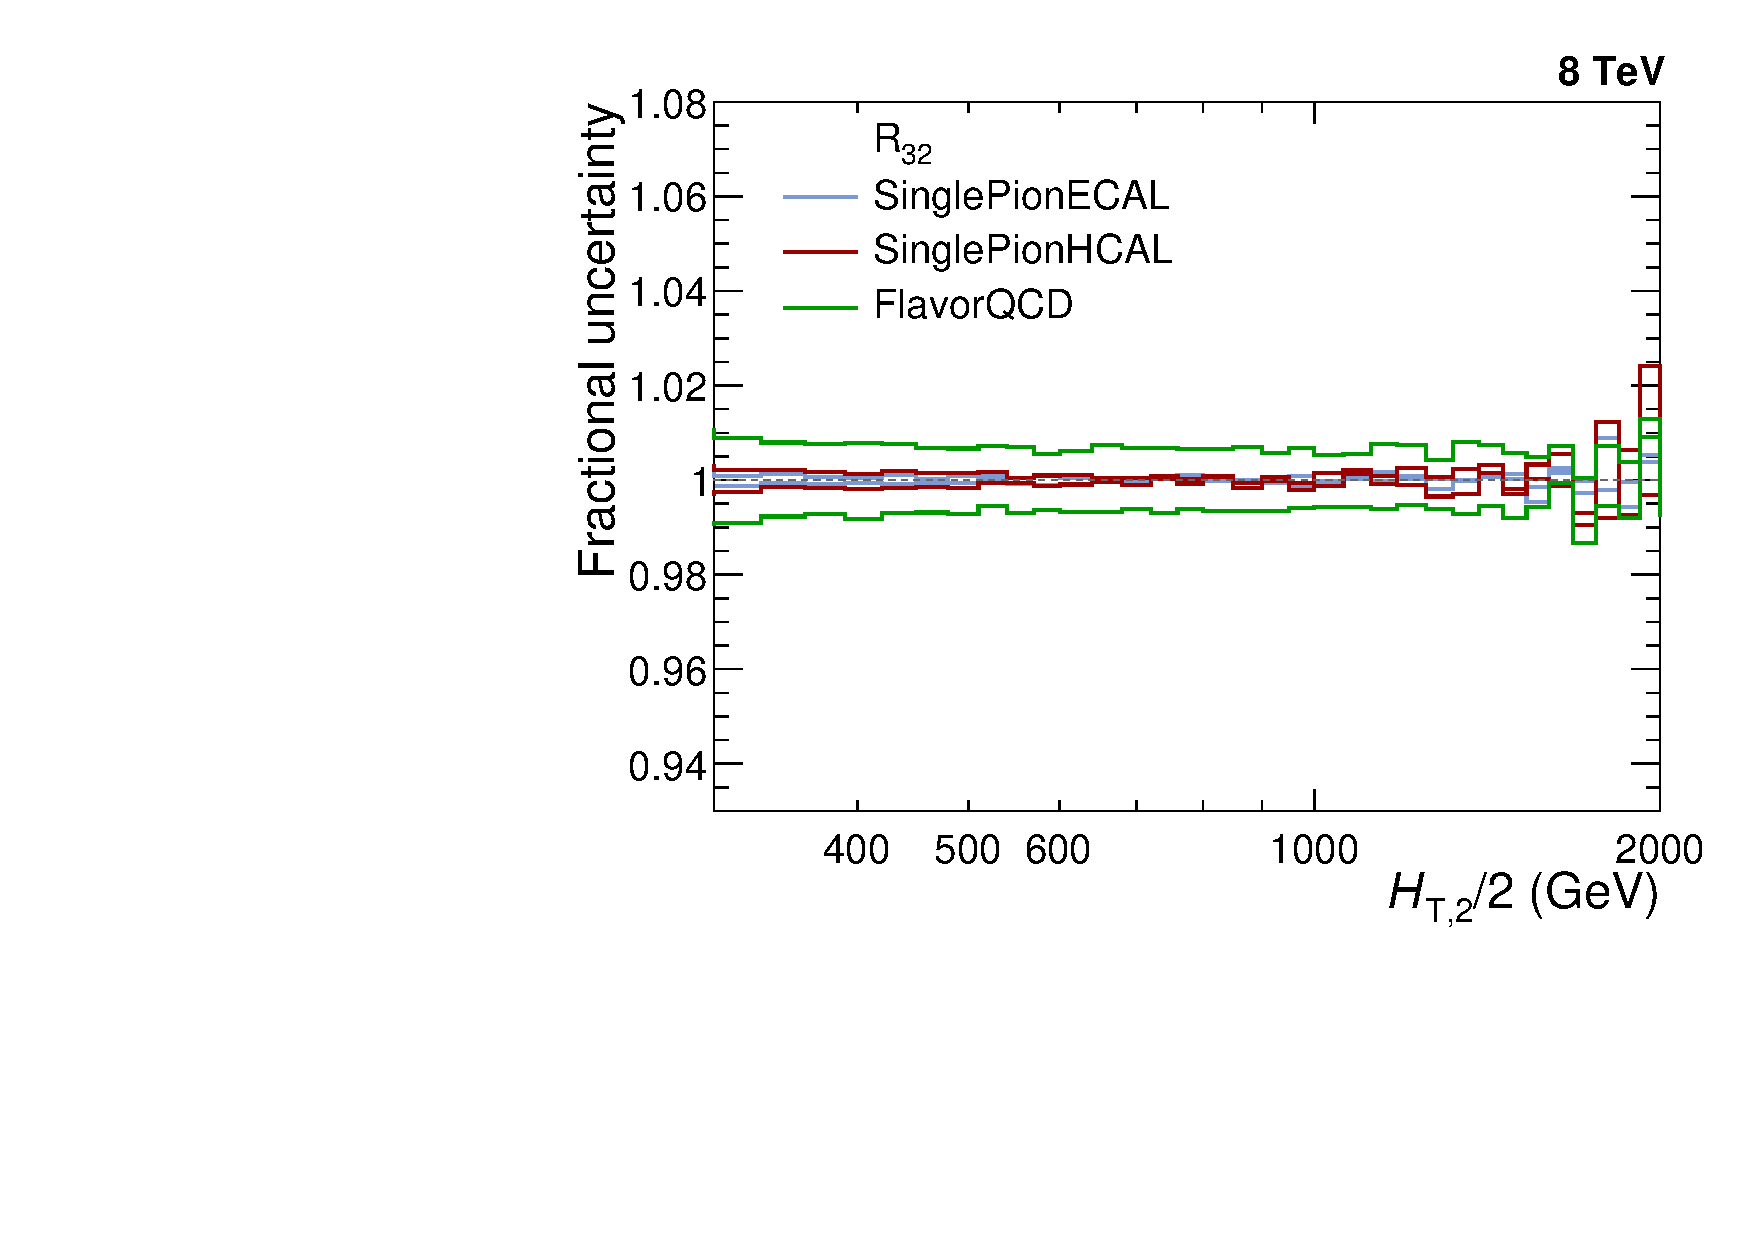
\includegraphics[width=0.51\textwidth]{/home/anter/Desktop/Thesis/Plots_HT_2_150/Single/MC_Macro_Plot_Ratio_32_HT_2_Unc_Single_1.pdf}
\caption[The fractional jet energy correction (JEC) uncertainties from individual sources (Part I).]{The fractional jet energy correction (JEC) uncertainties from individual sources are shown for inclusive 2-jet (top) and 3-jet (middle) events cross-sections and the cross-section ratio \ratio (bottom). On left, JEC uncertainties are evaluated from AbsoluteStat (blue), AbsoluteScale (red), AbsoluteMPFBias (green) and Fragmentation (pink) sources whereas on right, these are evaluated from SinglePionECAL (blue), SinglePionHCAL (red) and FlavorQCD (green) sources.}
\label{fig:jes1}
%\end{center}
\end{figure}

\begin{figure}[!hbtp]
%\begin{center}
\hspace*{-5mm}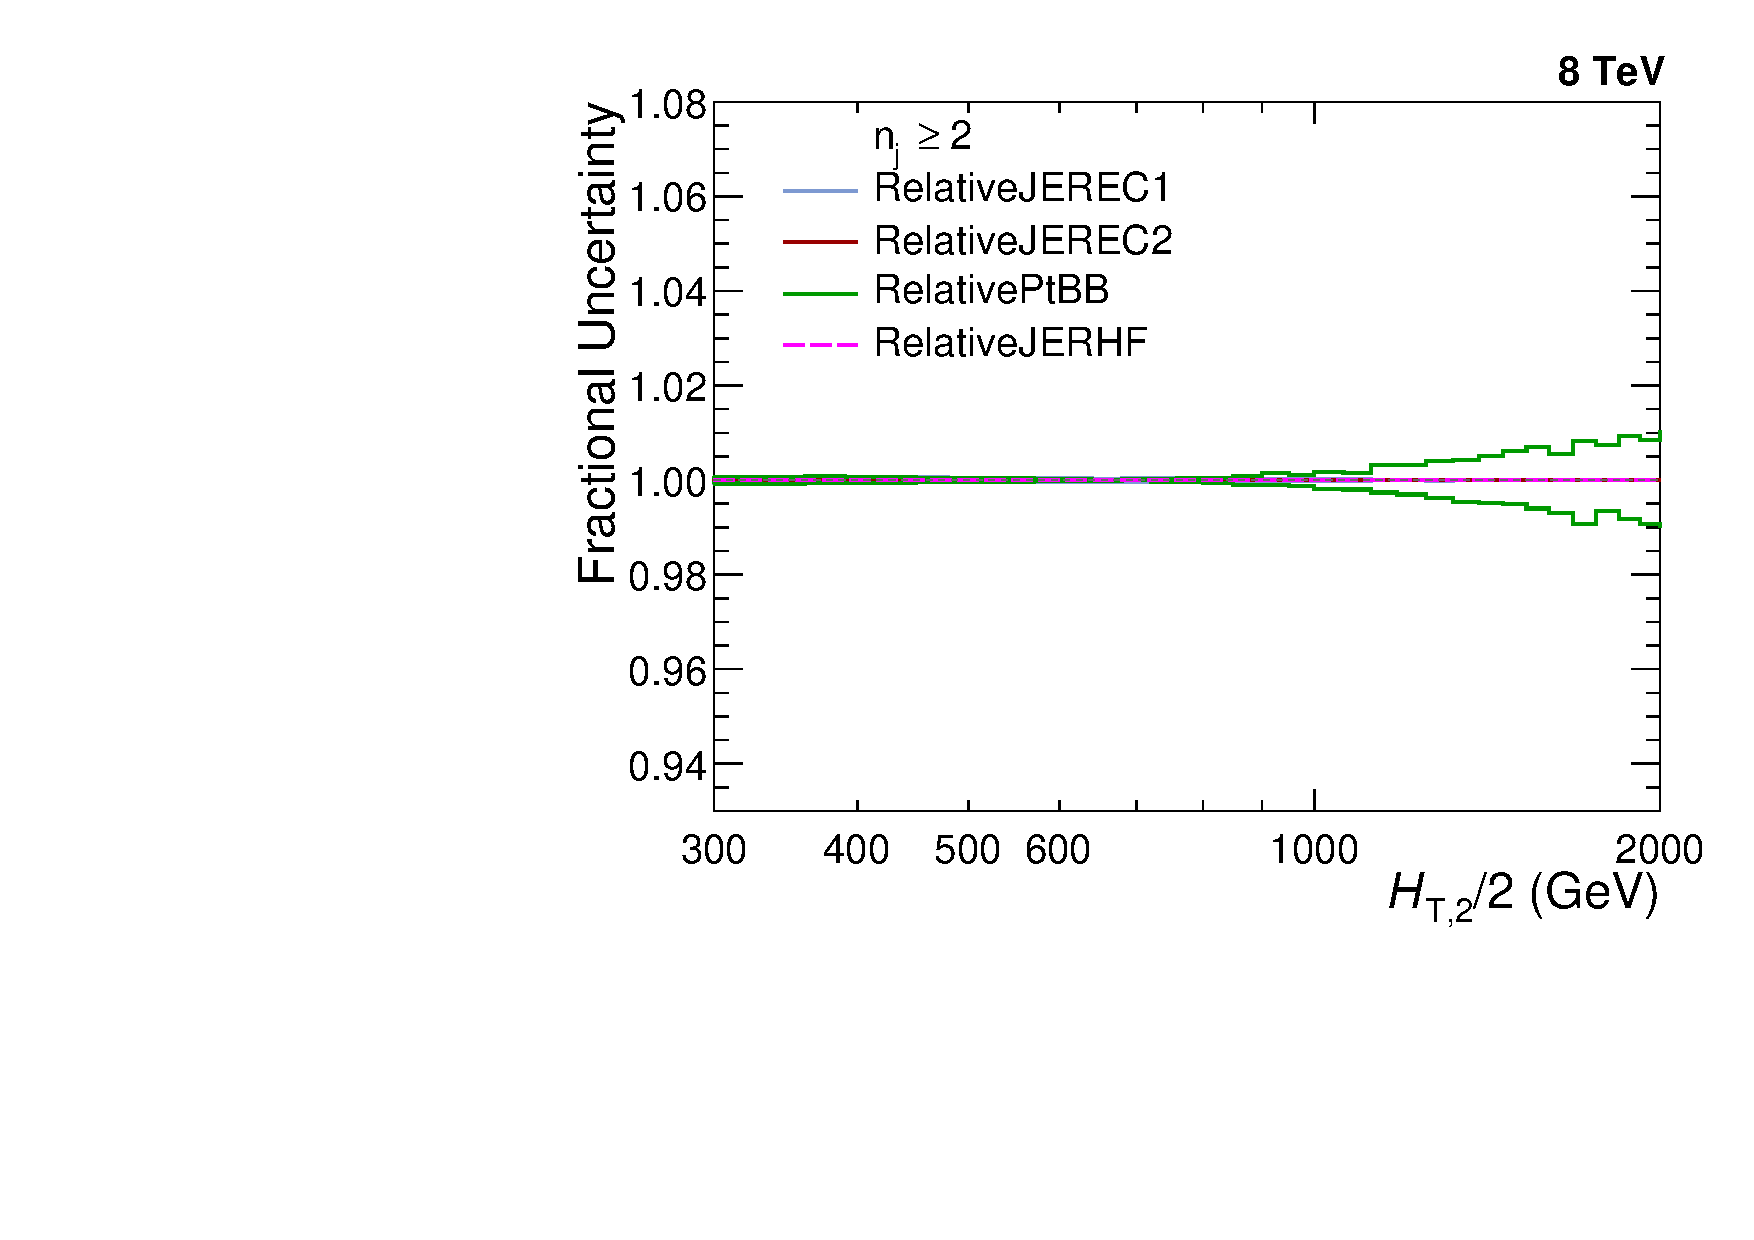
\includegraphics[width=0.51\textwidth]{/home/anter/Desktop/Thesis/Plots_HT_2_150/Single/MC_Macro_Plot_All_2_HT_2_Unc_Relative_1.pdf}%
~~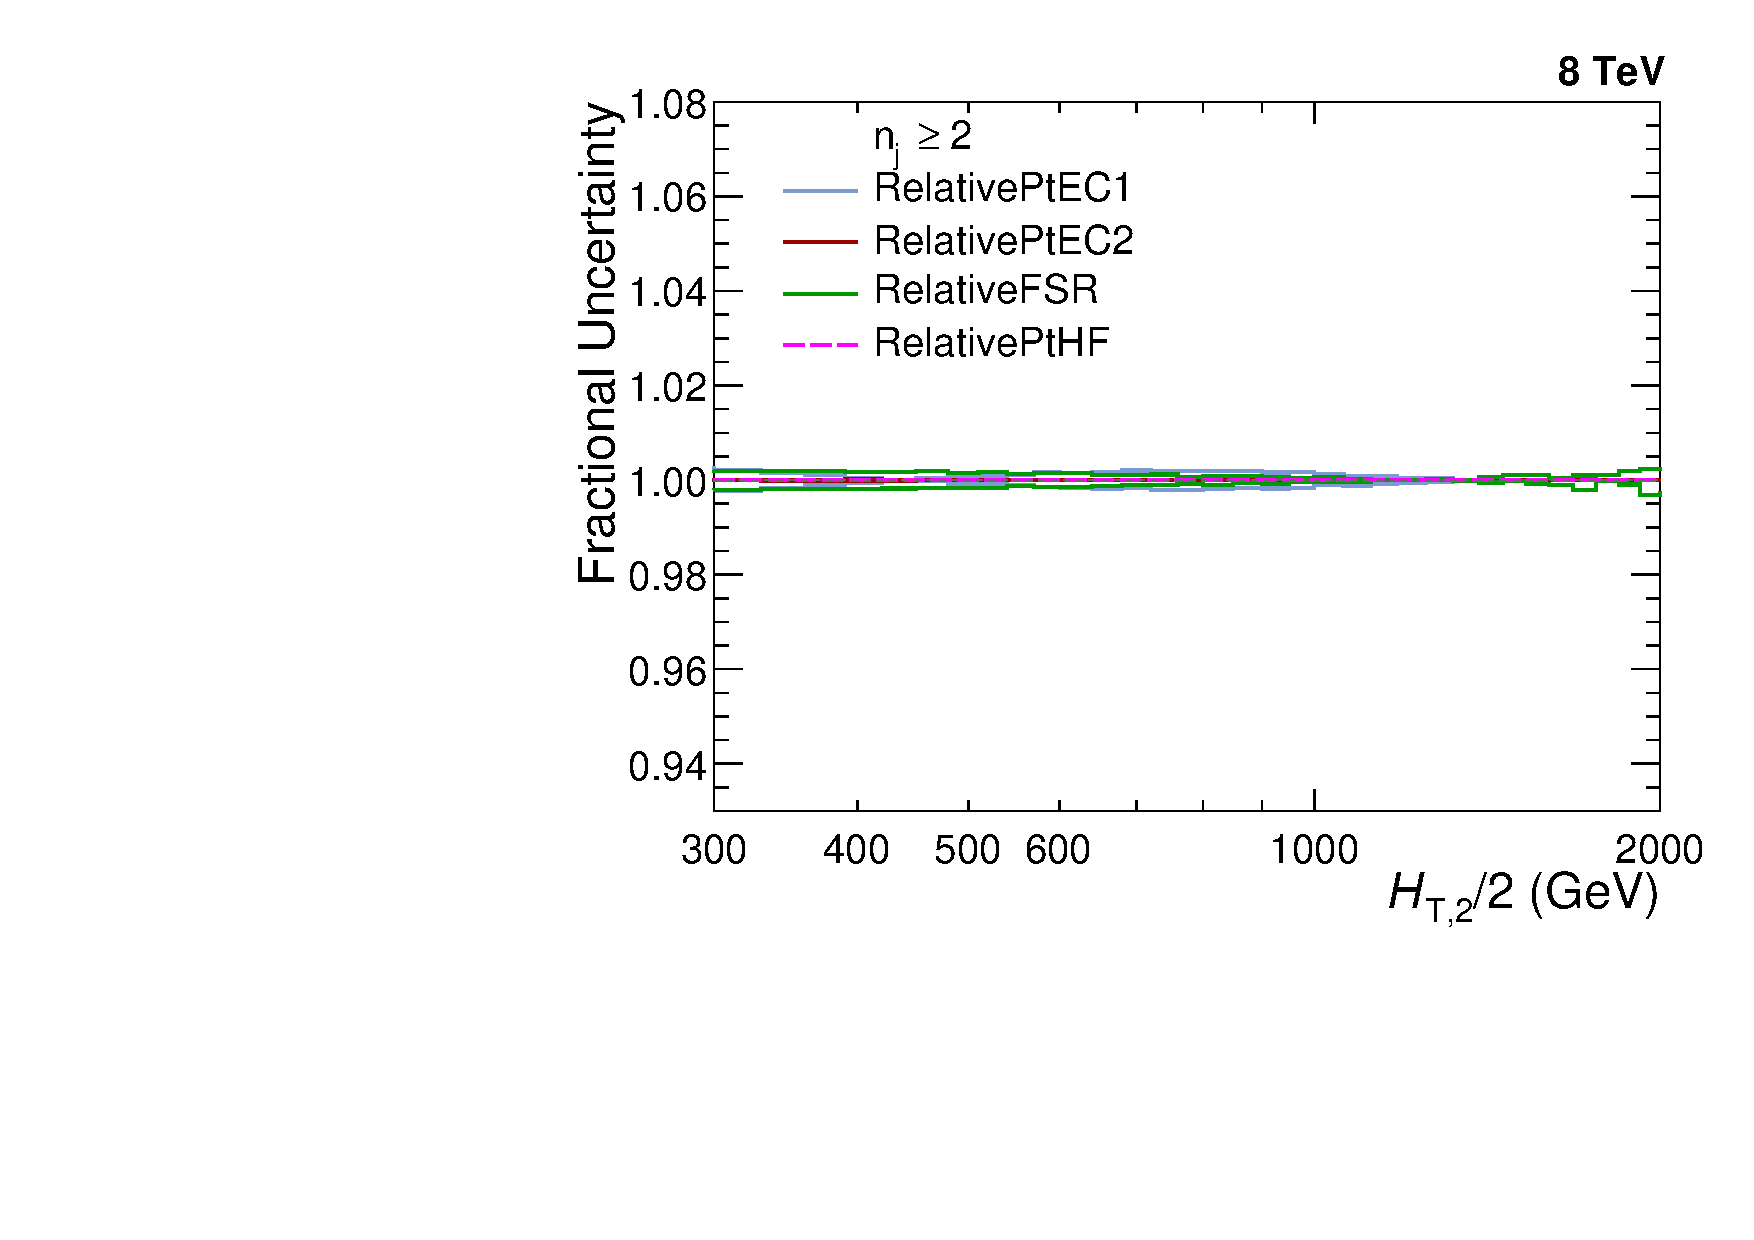
\includegraphics[width=0.51\textwidth]{/home/anter/Desktop/Thesis/Plots_HT_2_150/Single/MC_Macro_Plot_All_2_HT_2_Unc_Relative_2.pdf}\\
\hspace*{-5mm}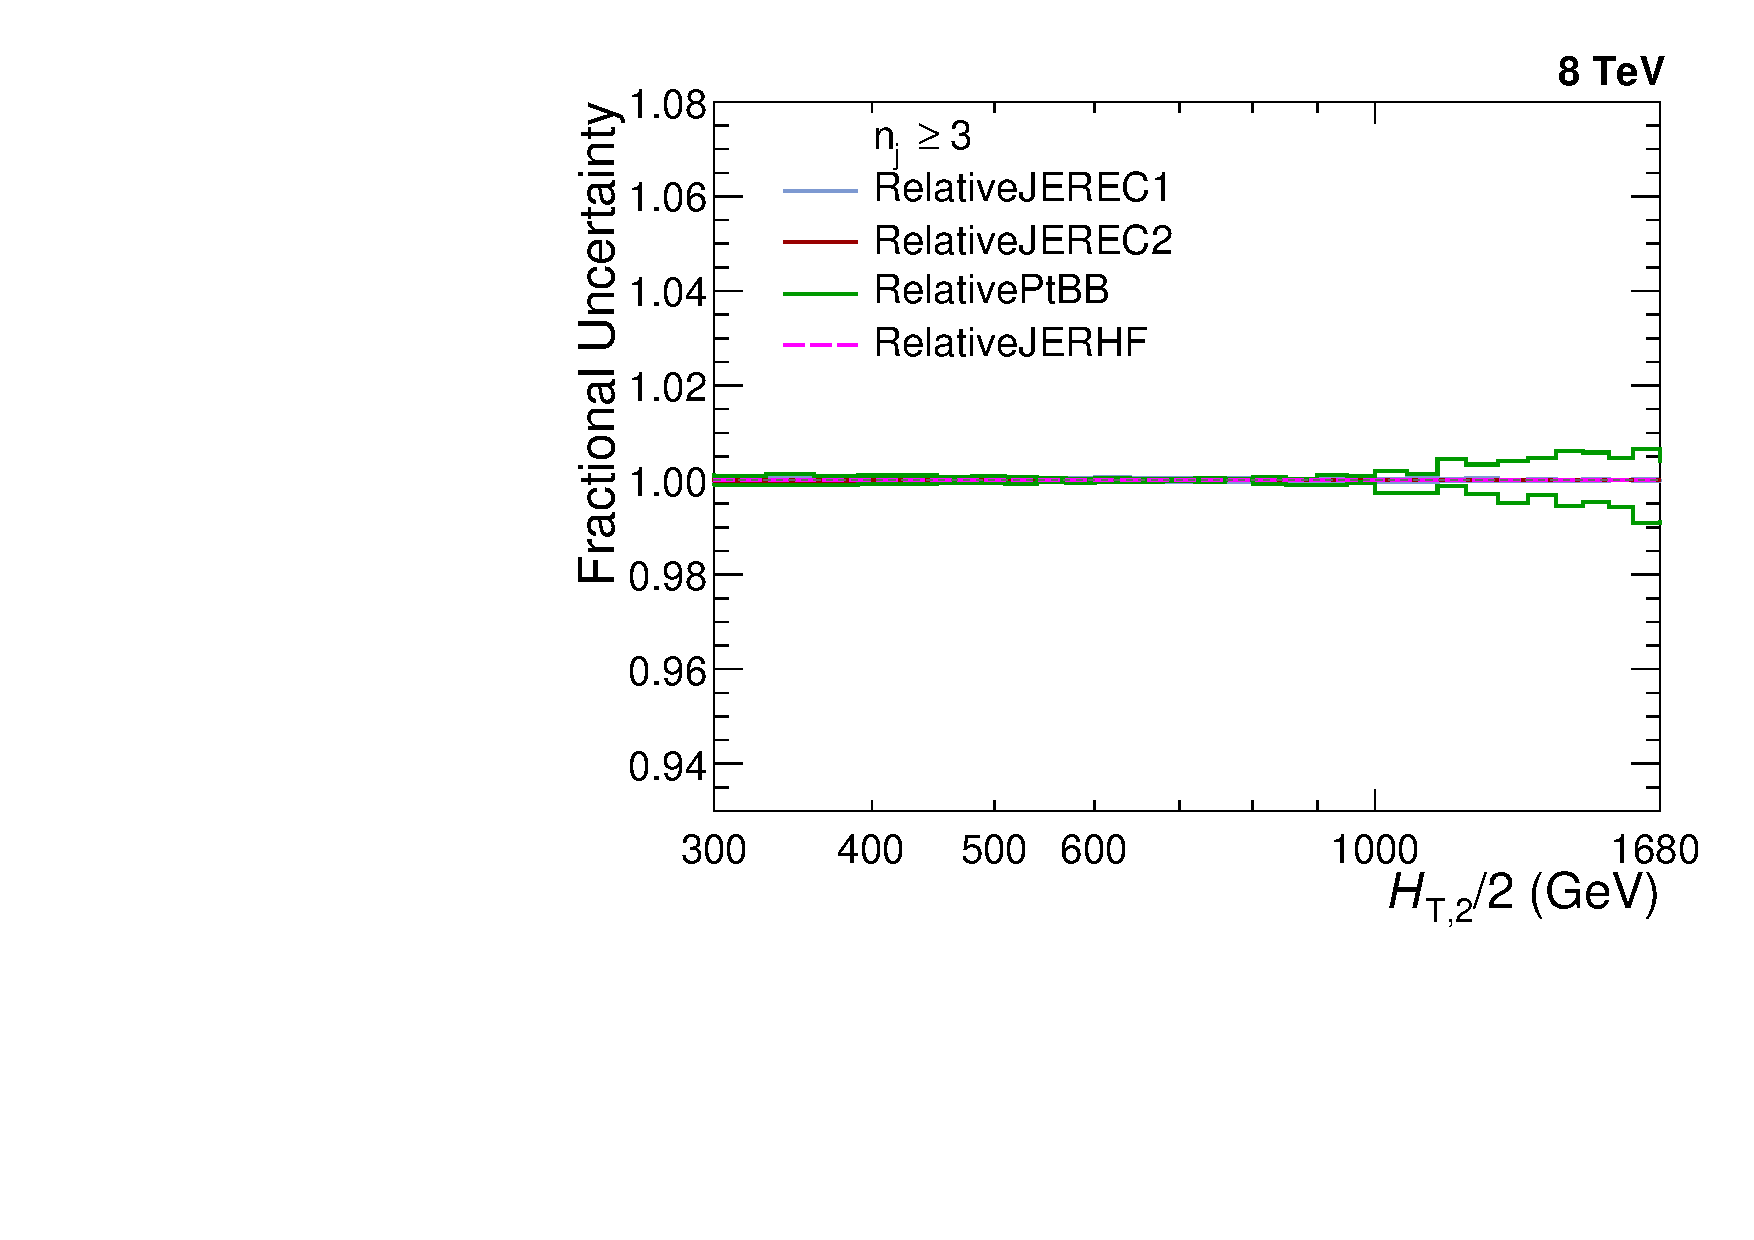
\includegraphics[width=0.51\textwidth]{/home/anter/Desktop/Thesis/Plots_HT_2_150/Single/MC_Macro_Plot_All_3_HT_2_Unc_Relative_1.pdf}%
~~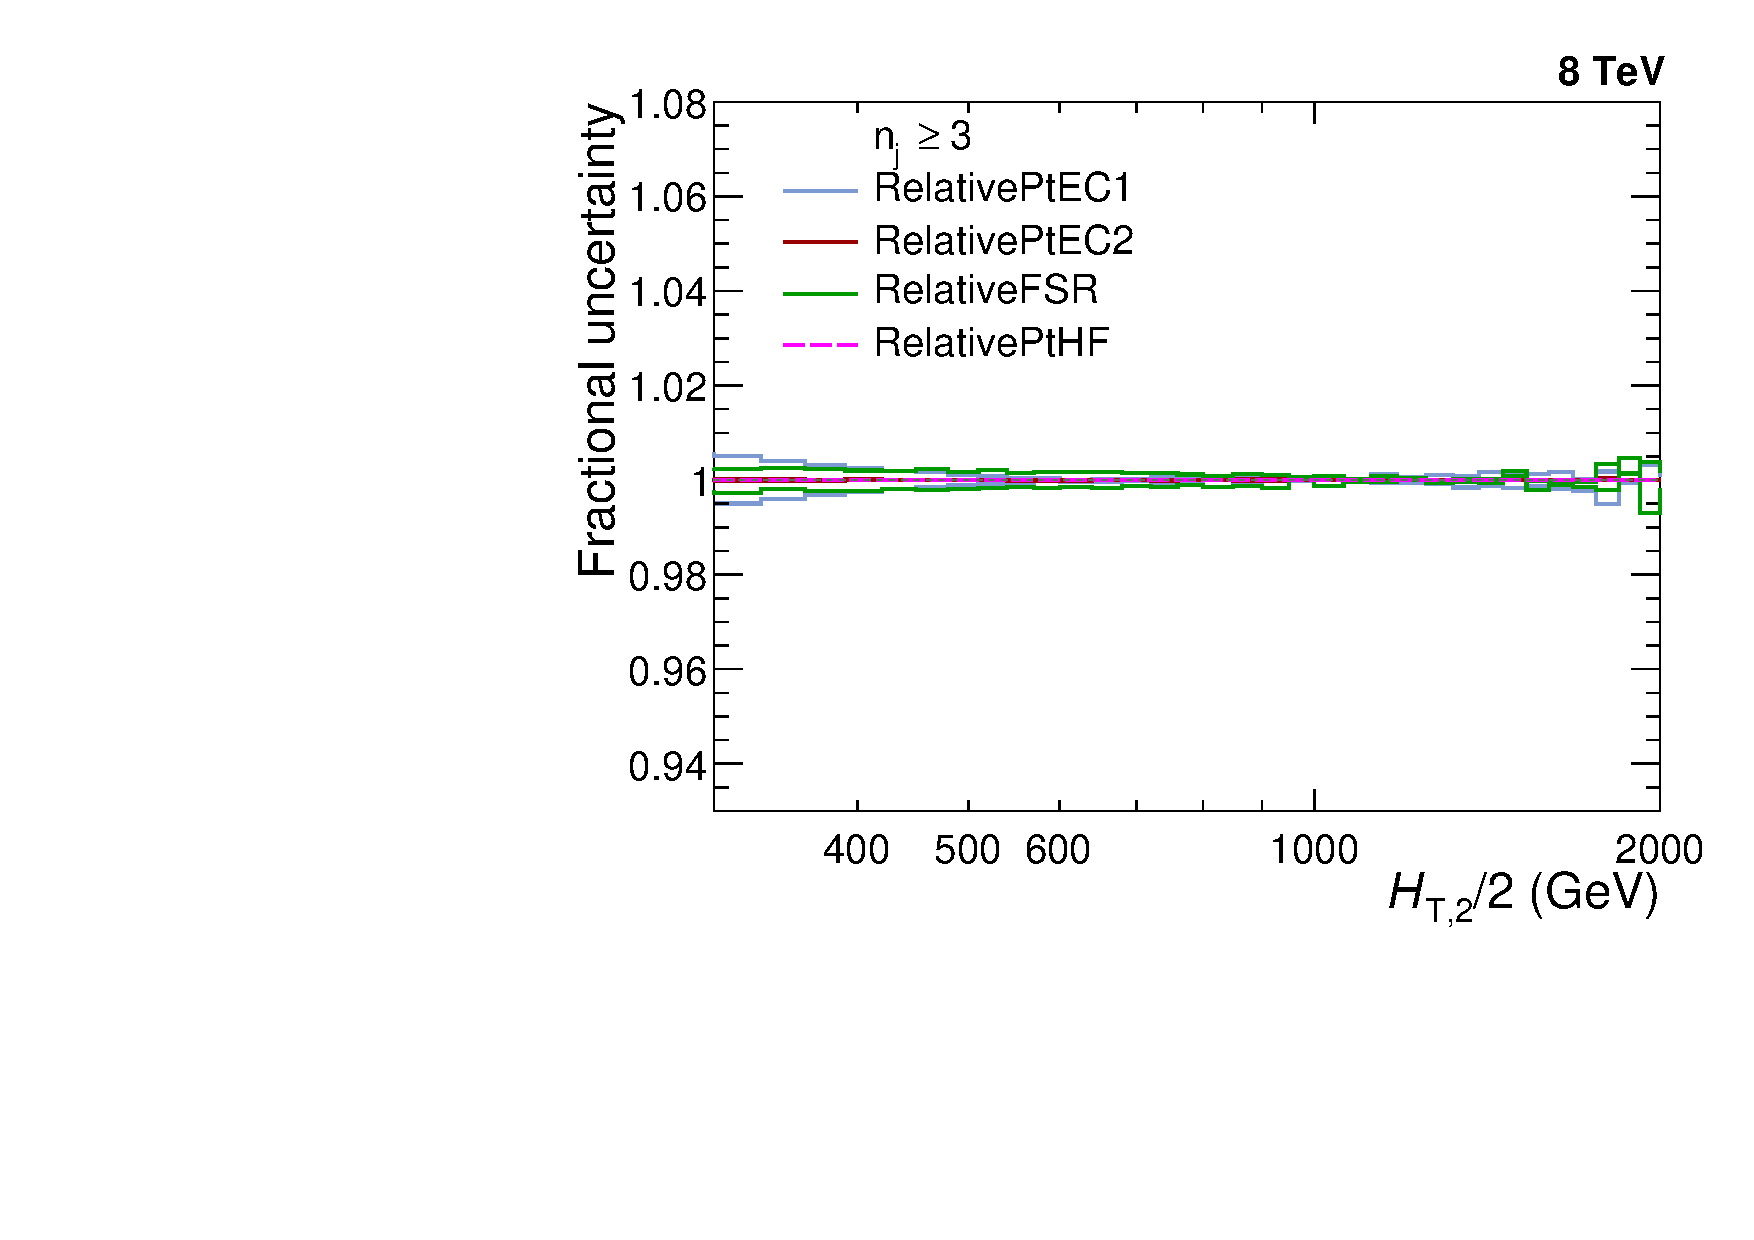
\includegraphics[width=0.51\textwidth]{/home/anter/Desktop/Thesis/Plots_HT_2_150/Single/MC_Macro_Plot_All_3_HT_2_Unc_Relative_2.pdf}\\
\hspace*{-5mm}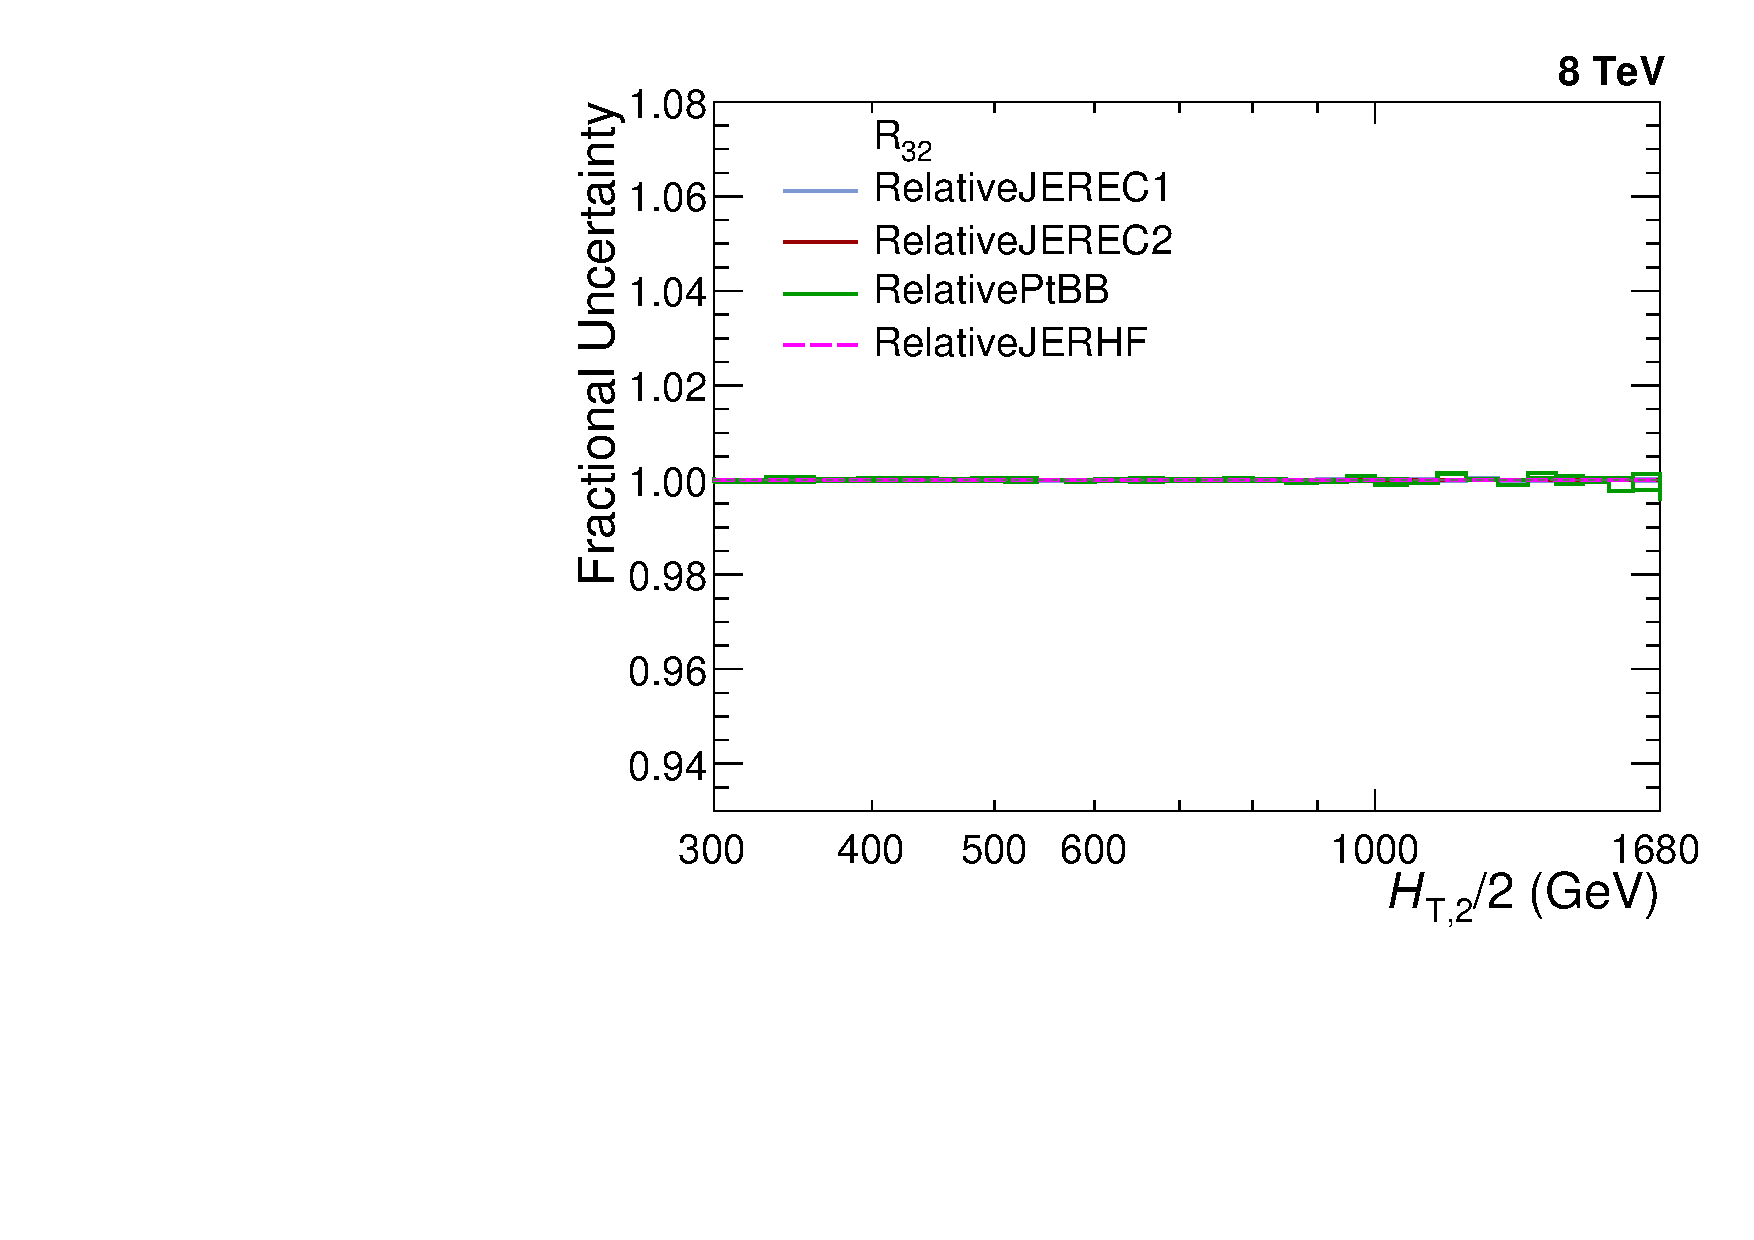
\includegraphics[width=0.51\textwidth]{/home/anter/Desktop/Thesis/Plots_HT_2_150/Single/MC_Macro_Plot_Ratio_32_HT_2_Unc_Relative_1.pdf}%
~~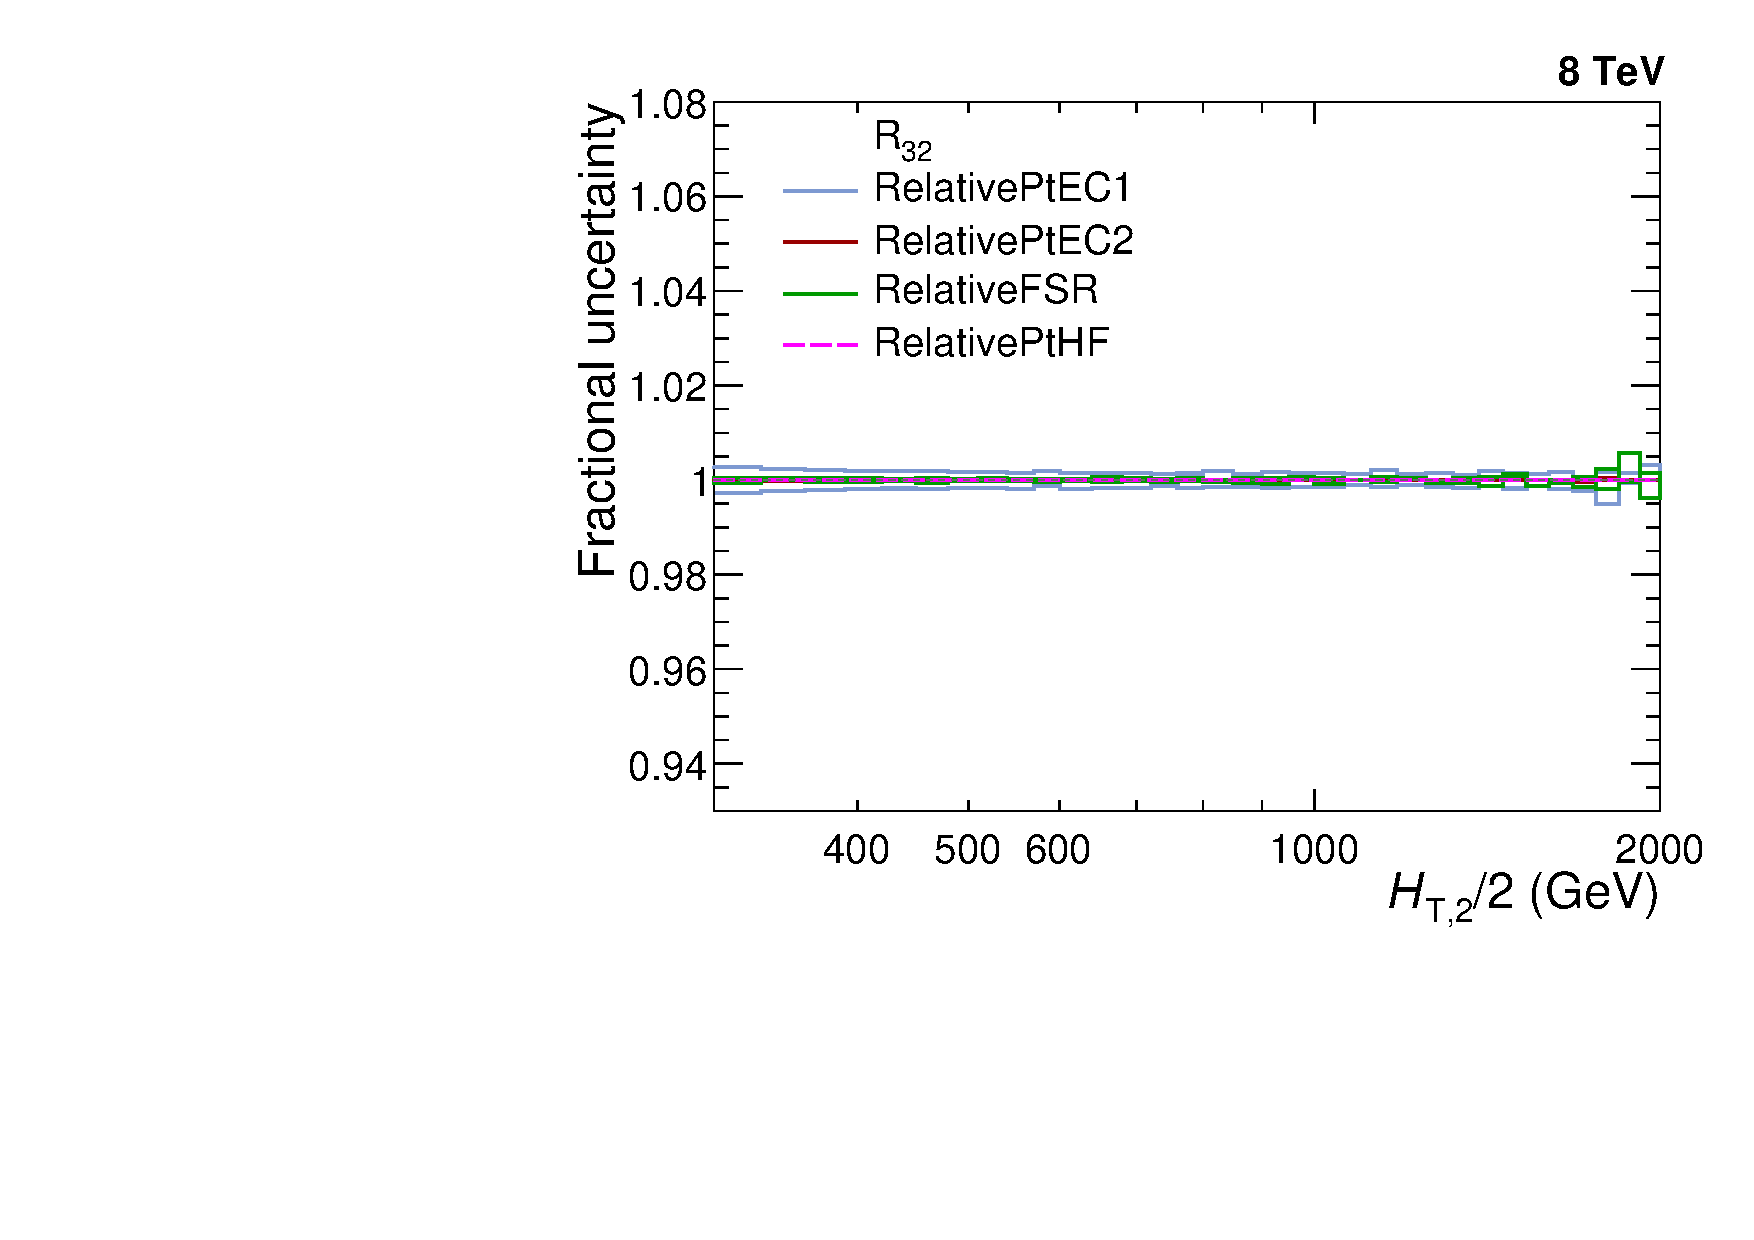
\includegraphics[width=0.51\textwidth]{/home/anter/Desktop/Thesis/Plots_HT_2_150/Single/MC_Macro_Plot_Ratio_32_HT_2_Unc_Relative_2.pdf}
\caption[The fractional jet energy correction (JEC) uncertainties from individual sources (Part II).]{The fractional jet energy correction (JEC) uncertainties from individual sources are shown for inclusive 2-jet (top) and 3-jet (middle) events cross-sections and the cross-section ratio \ratio (bottom). On left, JEC uncertainties are evaluated from RelativeJEREC1 (blue), RelativeJEREC2 (red), RelativePtBB (green) and RelativeJERHF (pink) sources whereas on right, these are evaluated from RelativePtEC1 (blue), RelativePtEC2 (red), RelativePFSR (green) and RelativePtHF (pink) sources.}
\label{fig:jes2}
%\end{center}
\end{figure}

\begin{figure}[!hbtp]
%\begin{center}
\hspace*{-5mm}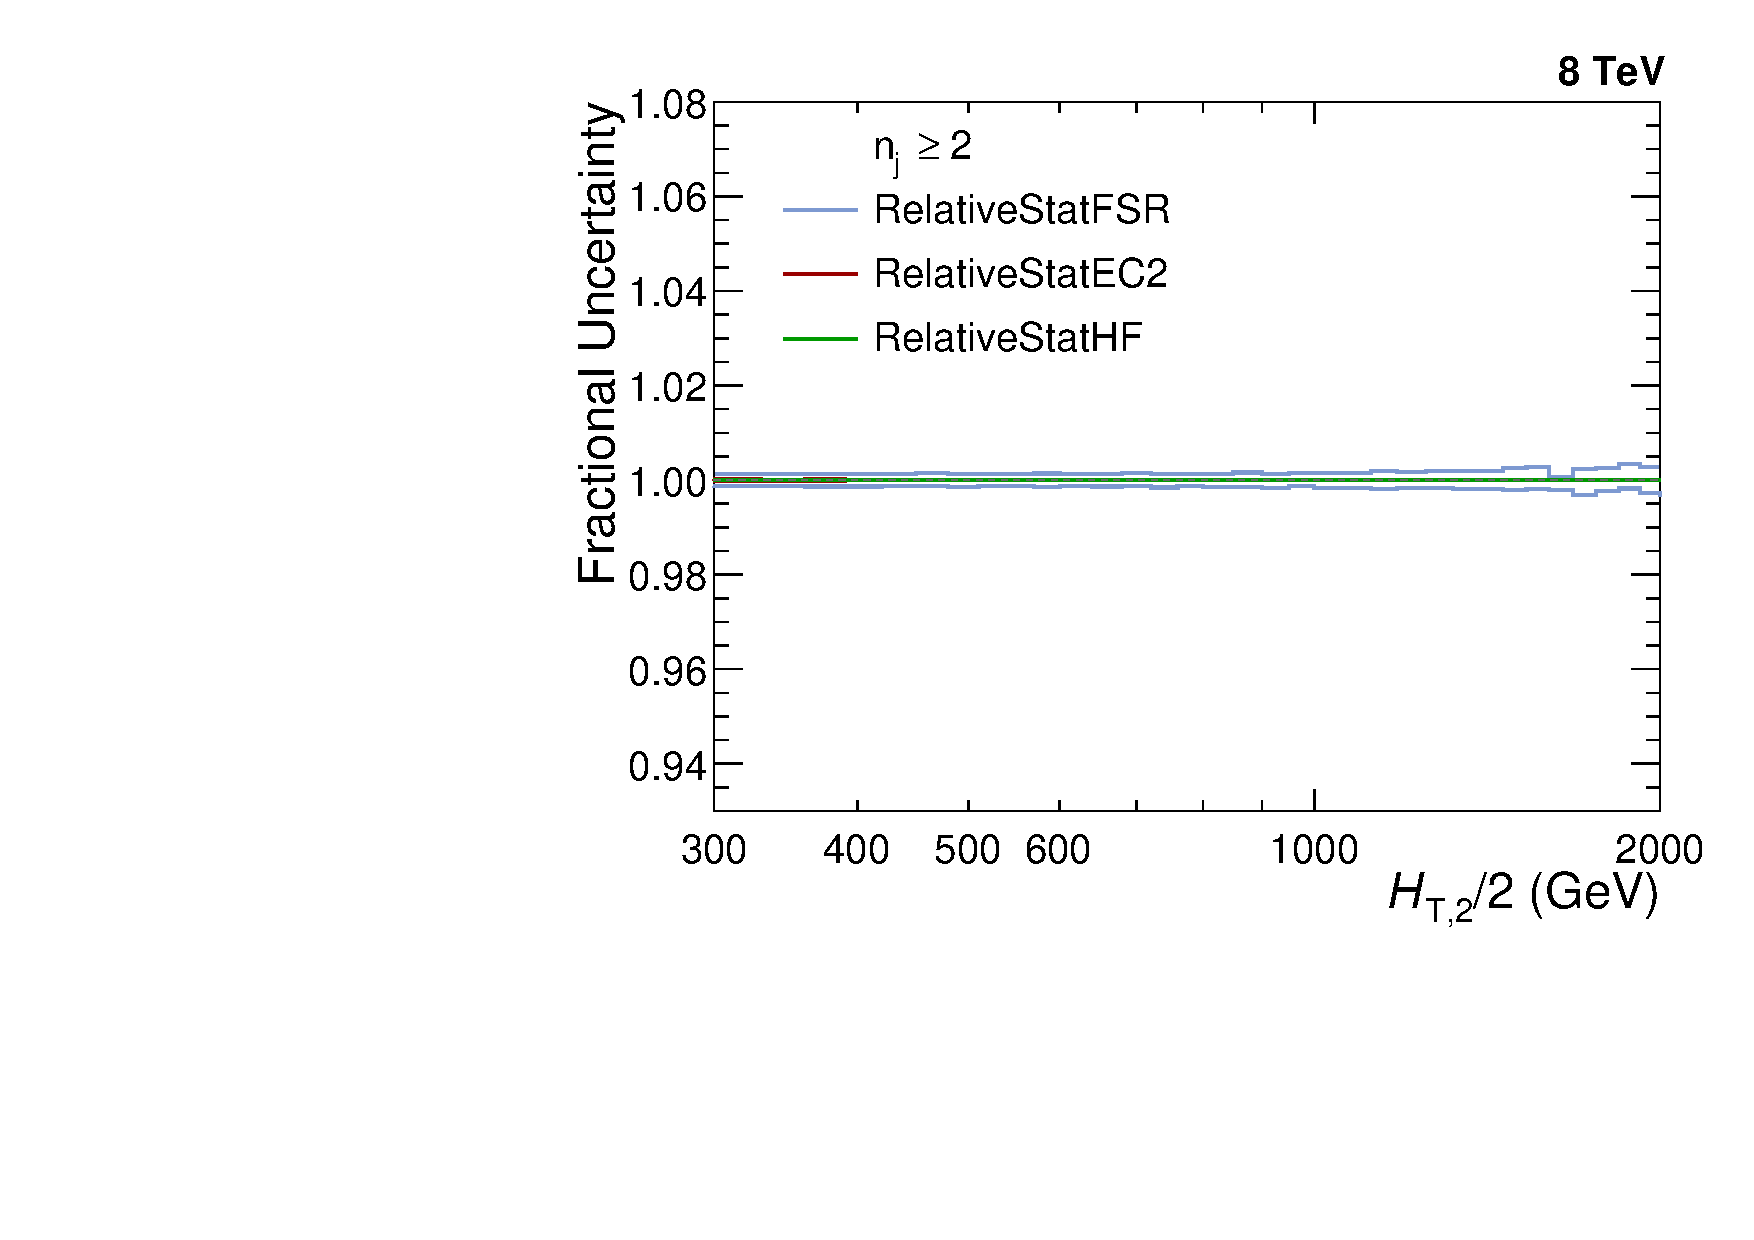
\includegraphics[width=0.51\textwidth]{/home/anter/Desktop/Thesis/Plots_HT_2_150/Single/MC_Macro_Plot_All_2_HT_2_Unc_RelativeStat_1.pdf}%
~~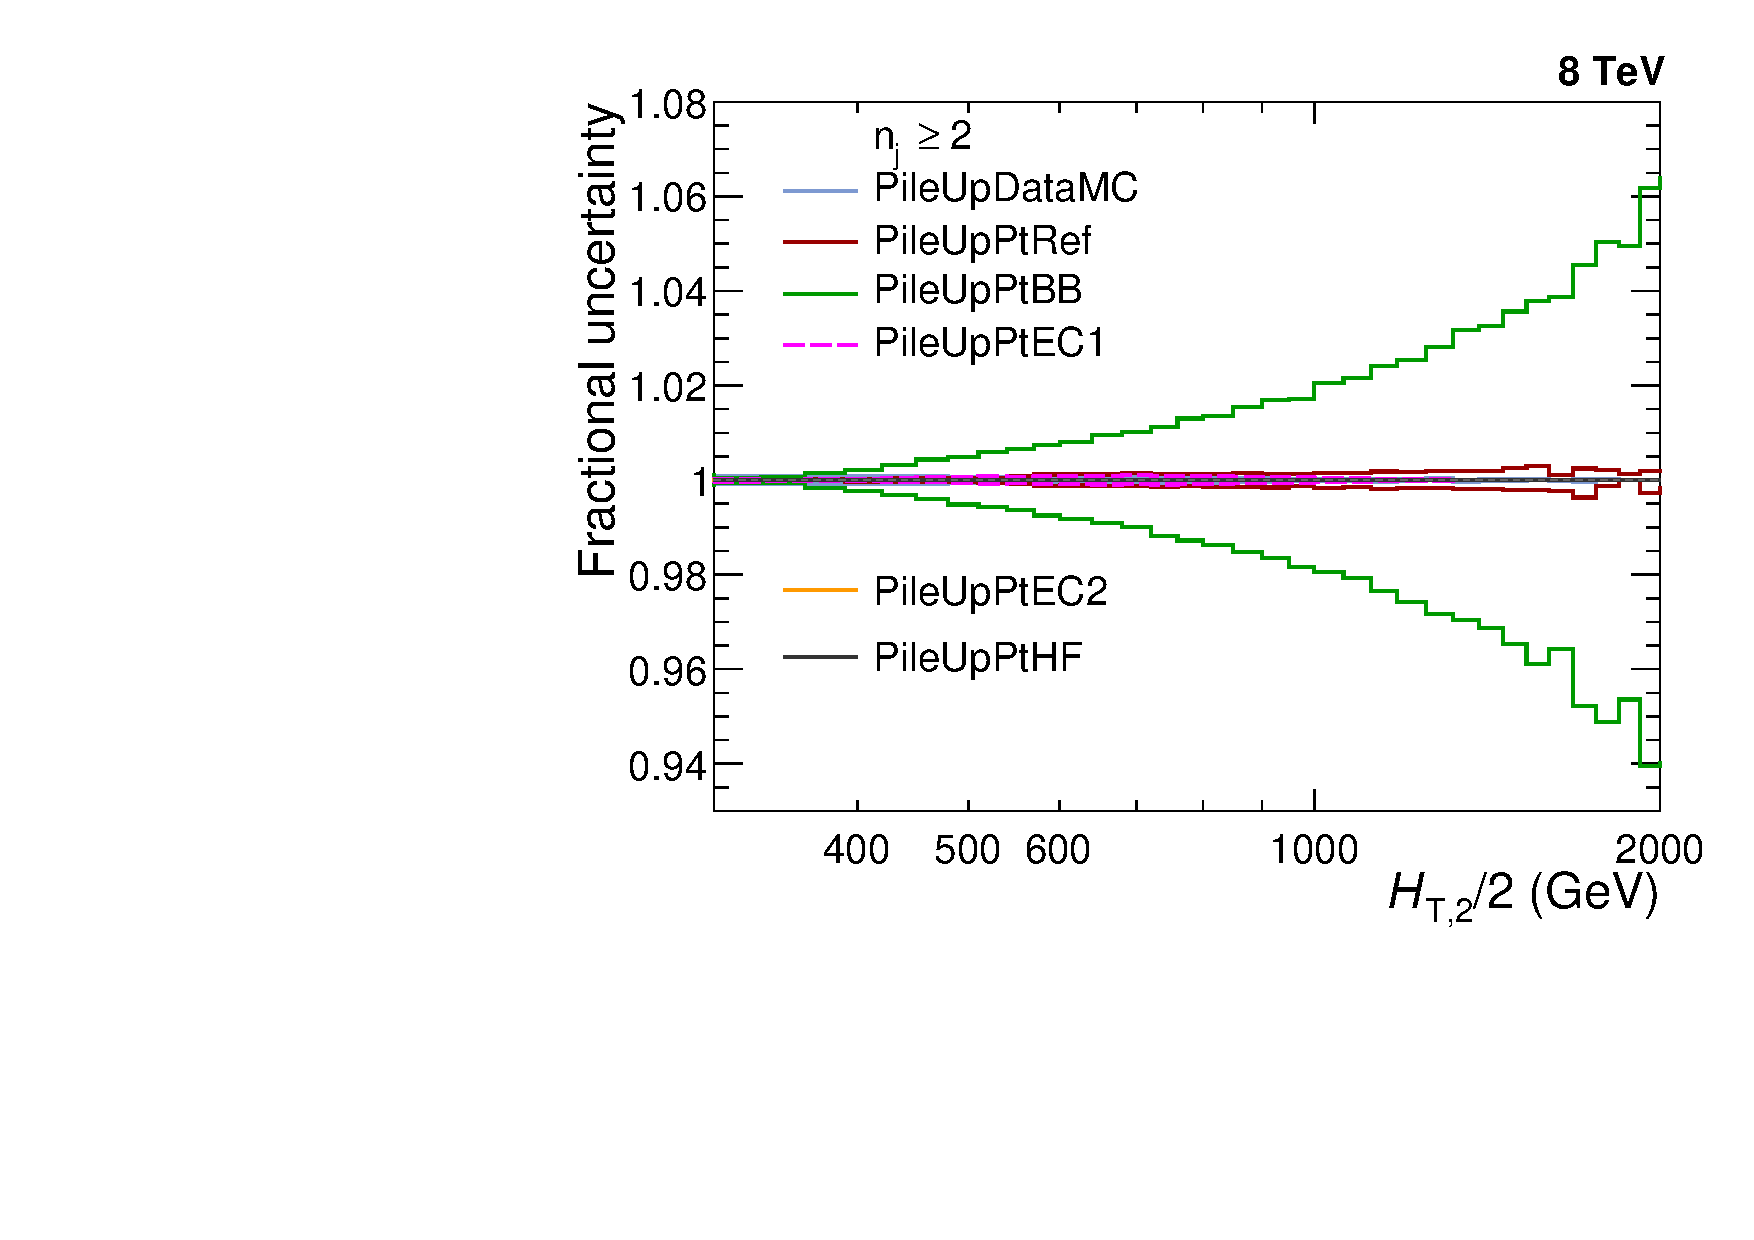
\includegraphics[width=0.51\textwidth]{/home/anter/Desktop/Thesis/Plots_HT_2_150/Single/MC_Macro_Plot_All_2_HT_2_Unc_Pileup_1.pdf}\\
\hspace*{-5mm}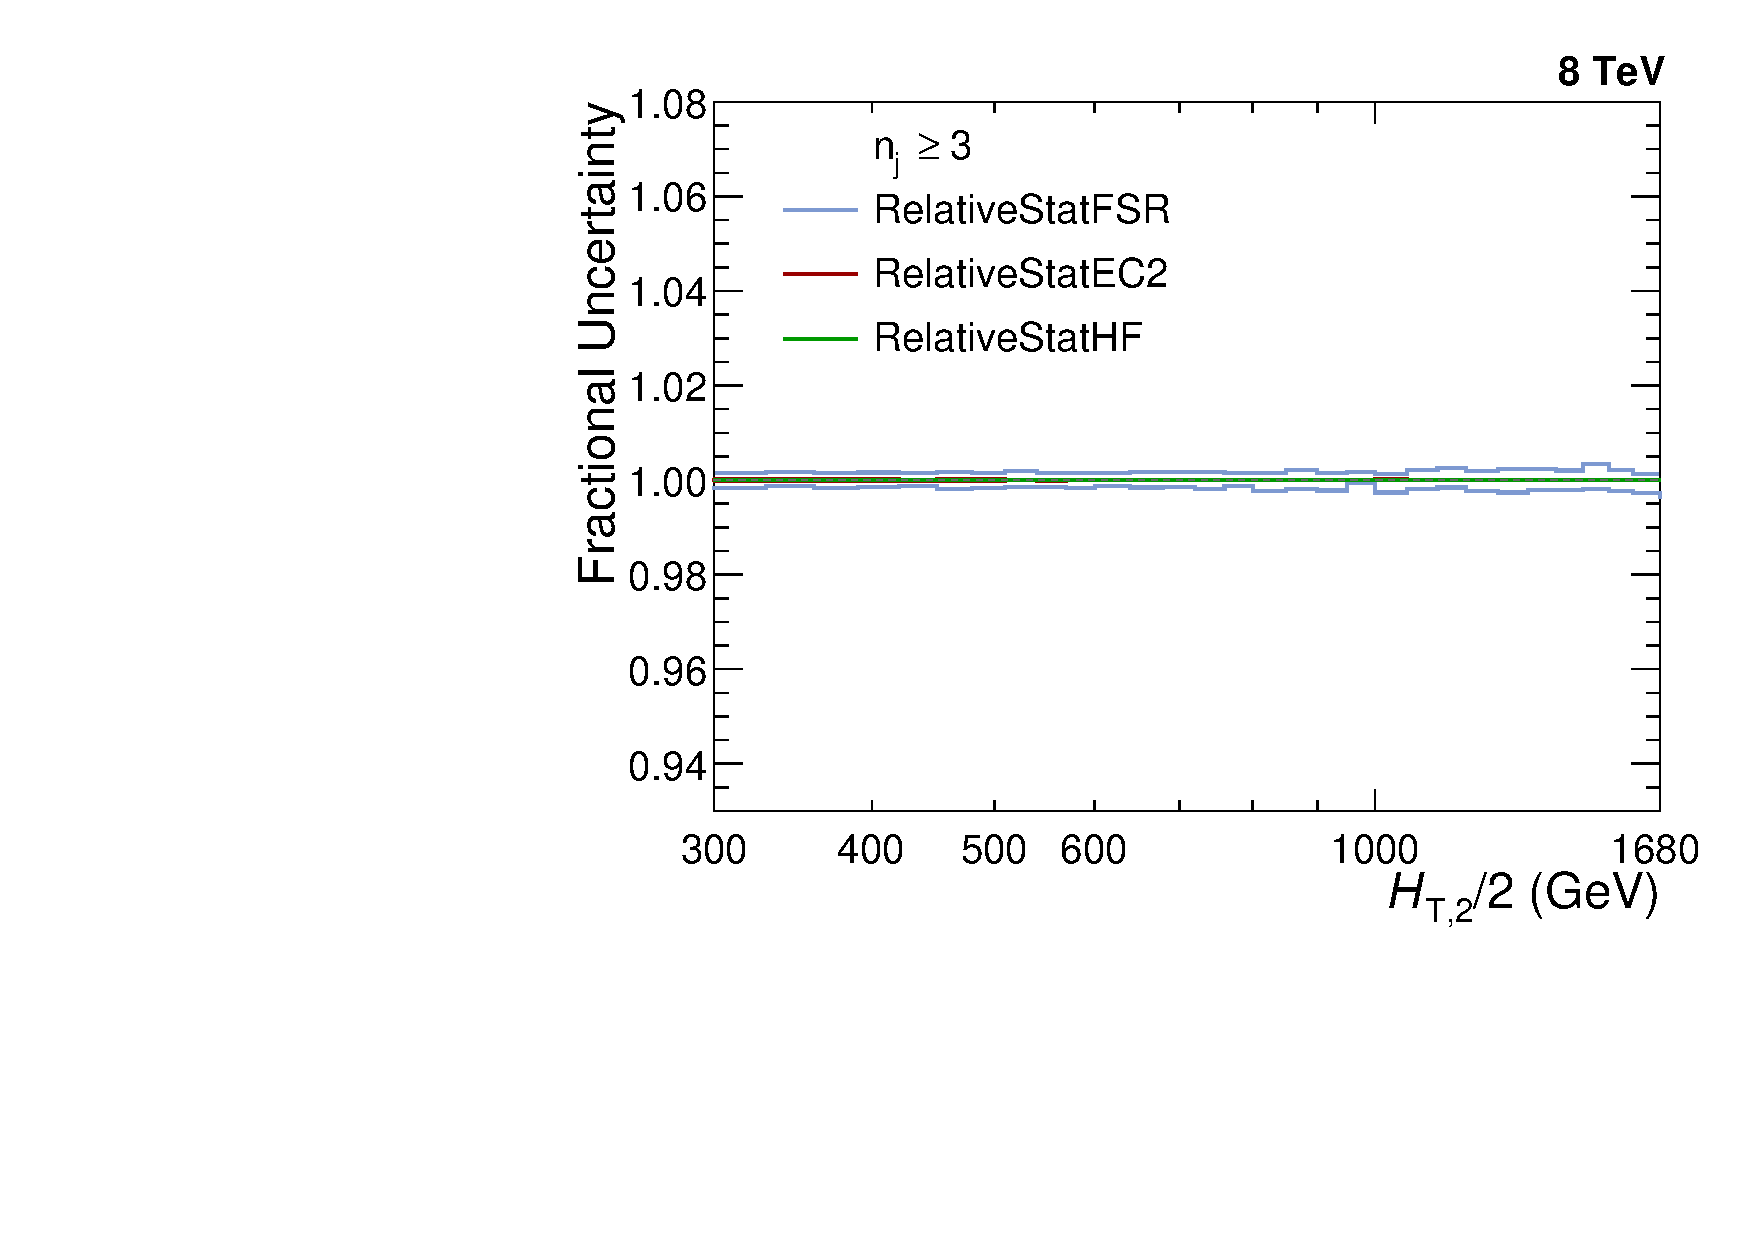
\includegraphics[width=0.51\textwidth]{/home/anter/Desktop/Thesis/Plots_HT_2_150/Single/MC_Macro_Plot_All_3_HT_2_Unc_RelativeStat_1.pdf}%
~~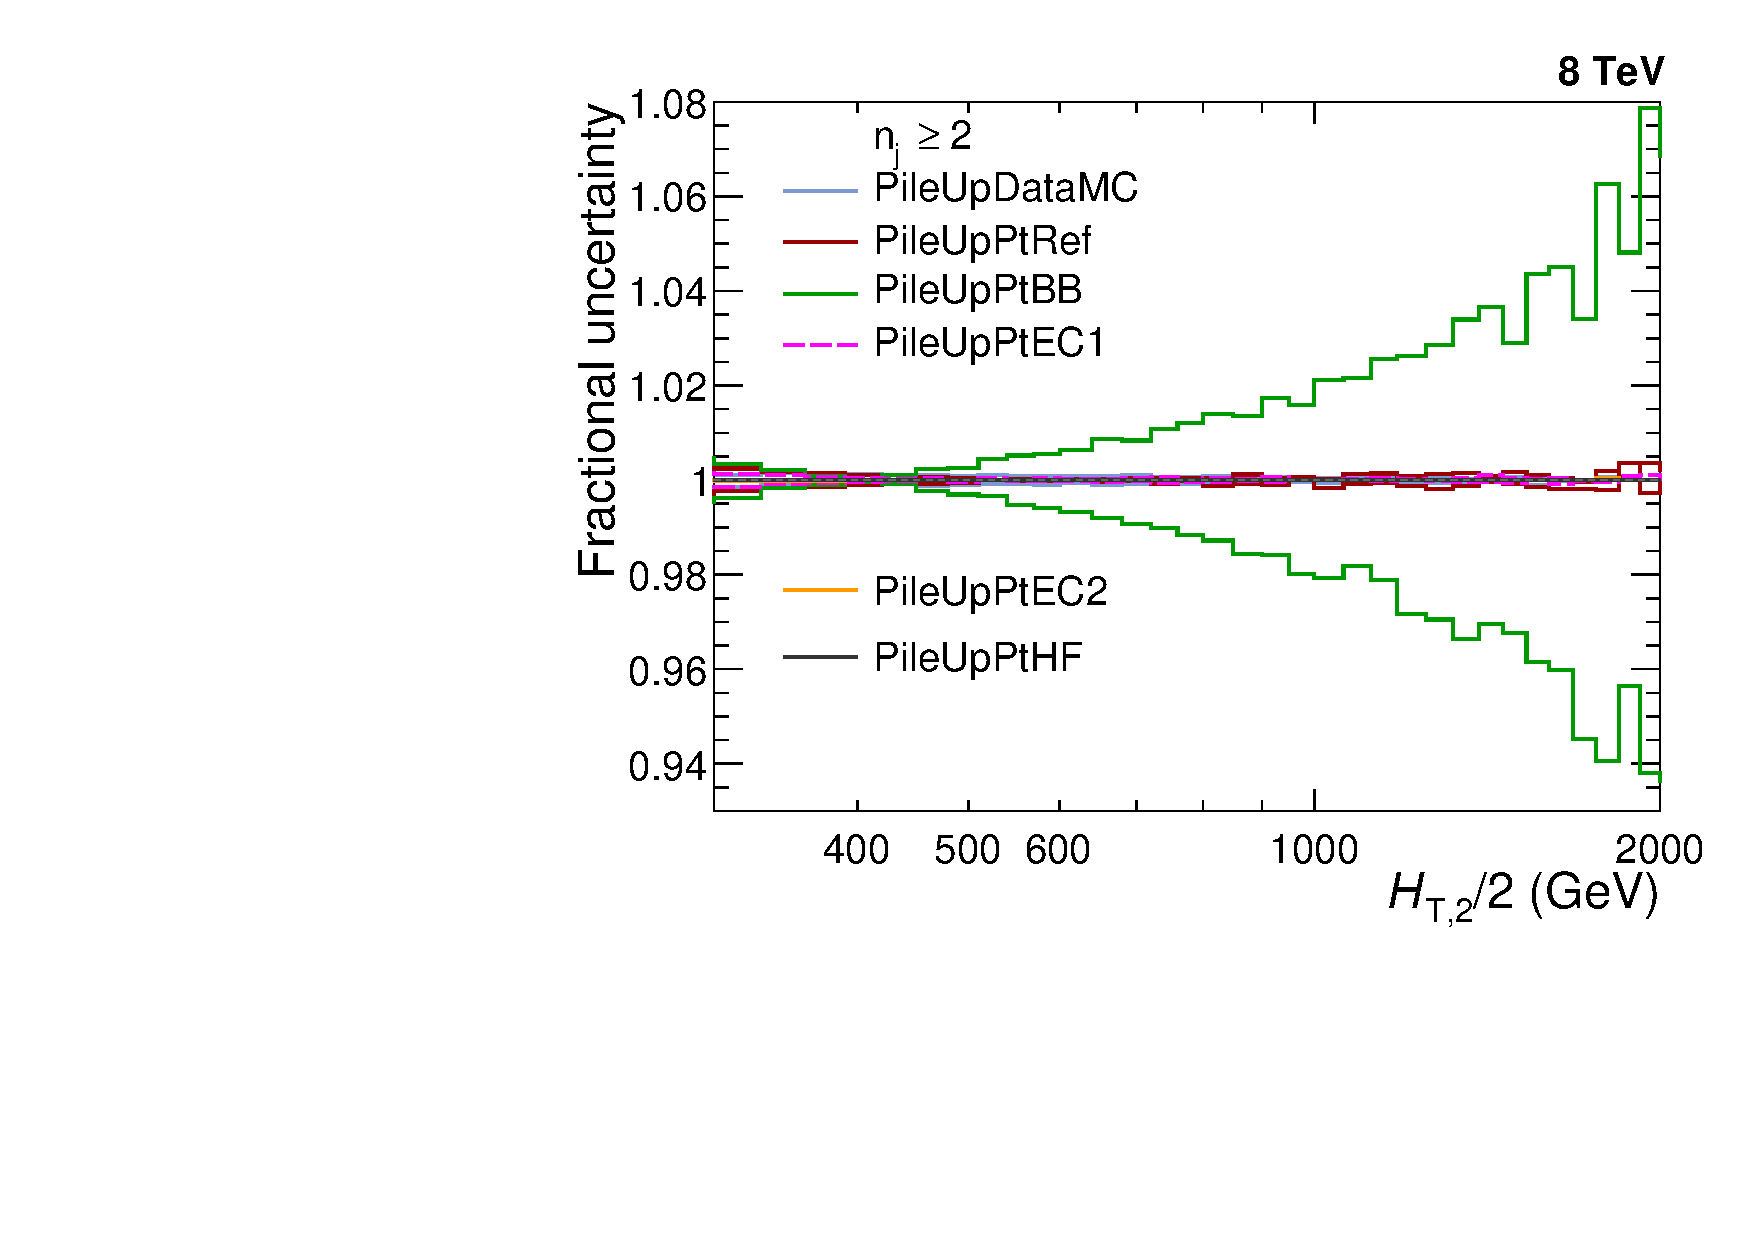
\includegraphics[width=0.51\textwidth]{/home/anter/Desktop/Thesis/Plots_HT_2_150/Single/MC_Macro_Plot_All_3_HT_2_Unc_Pileup_1.pdf}\\
\hspace*{-5mm}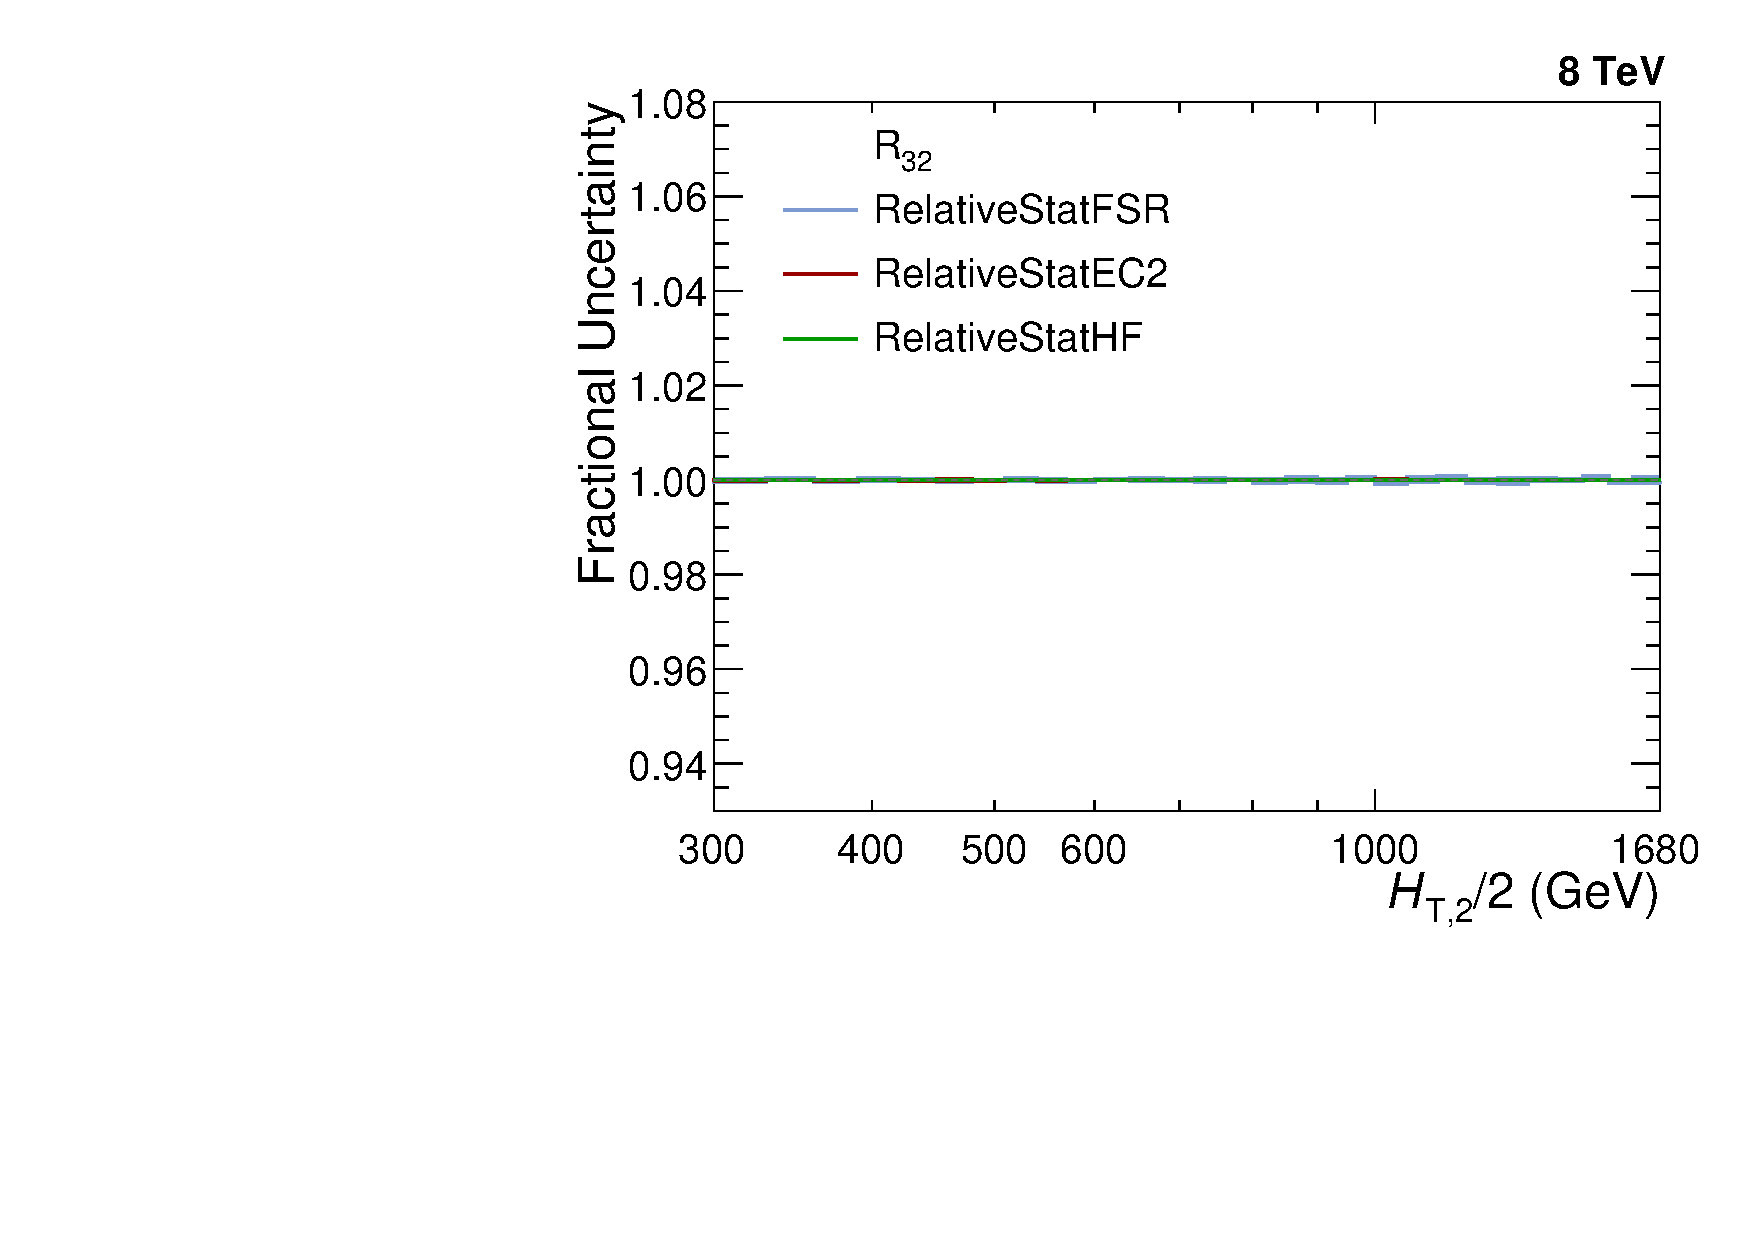
\includegraphics[width=0.51\textwidth]{/home/anter/Desktop/Thesis/Plots_HT_2_150/Single/MC_Macro_Plot_Ratio_32_HT_2_Unc_RelativeStat_1.pdf}%
~~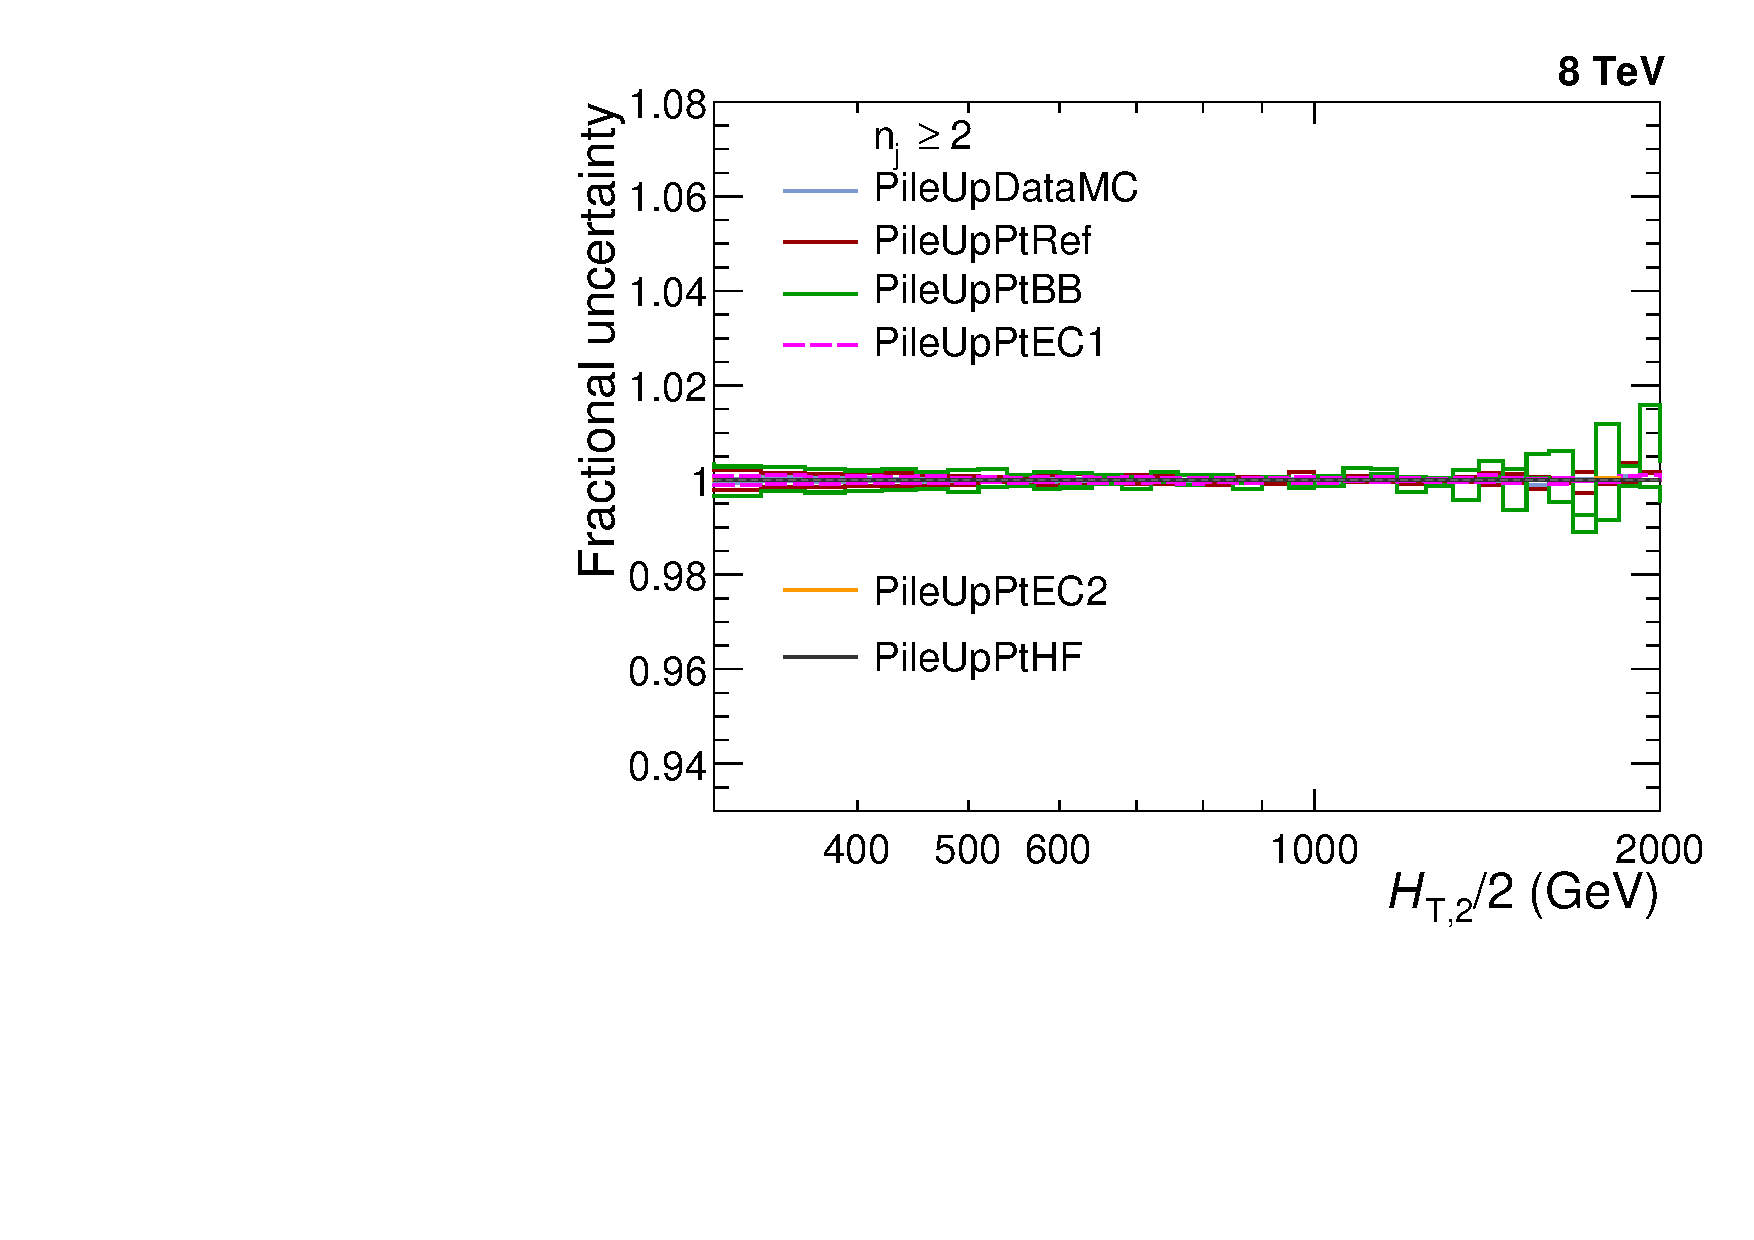
\includegraphics[width=0.51\textwidth]{/home/anter/Desktop/Thesis/Plots_HT_2_150/Single/MC_Macro_Plot_Ratio_32_HT_2_Unc_Pileup_1.pdf}
\caption[The fractional jet energy correction (JEC) uncertainties from individual sources (Part III).]{The fractional jet energy correction (JEC) uncertainties from individual sources are shown for inclusive 2-jet (top) and 3-jet (middle) events cross-sections and the cross-section ratio \ratio (bottom). On left, JEC uncertainties are evaluated from RelativeStatFSR (blue), RelativeStatEC2 (red) and RelativeStatHF (green) sources whereas on right, these are evaluated from PileUpDataMC (blue), PileUpPtRef (red), PileUpPtBB (green), PileUpPtEC1 (pink), PileUpPtEC2 (orange) and PileUpPtHF (black) sources.}
\label{fig:jes3}
%\end{center}
\end{figure}
\newpage
\section{Experimental Uncertainties}
\label{sec:Exp_unc}
\begin{table}[!htbp]
 \caption[Experimental uncertainties (in \%) affecting the cross-section measurement in each bin of \httwo for inclusive 2-jet events.]{Experimental uncertainties (in \%), from all sources as well as the total uncertainty, affecting the cross-section measurement in each bin of \httwo for inclusive 2-jet events.}
 \label{tab:exp_unc2}
 \centering
 \vspace{2mm}
 \begin{tabular}{ccccccc} \hline \hline
 %& x-section & & & & & & \rbtrrnm \\ 
 %Bin & (x 10$^{-3}$ (pb/GeV)) & {\bf Statistical} & {\bf \textcolor{blue}{JEC}} & {\bf \textcolor{green} {Unfolding}} & {\bf \textcolor{myred}{Lumi}} & {\bf \textcolor{lightpurple} {Residual}} & {\bf Total} \rbtrrnm \\ \hline 
 %Bin & {\bf Statistical} & {\bf \textcolor{blue2}{JEC}} & {\bf \textcolor{green} {Unfolding}} & {\bf \textcolor{myred}{Lumi}} & {\bf \textcolor{lightpurple} {Residual}} & {\bf Total} \rbtrrnm \\ \hline 
 {\bf Bin} & {\bf Statistical} & {\bf JEC} & {\bf Unfolding} & {\bf Lumi} & {\bf Residual} & {\bf Total} \rbtrrnm \\ \hline 

300 - 330 & 0.242 & $^{+2.612}_{-2.565}$ & $^{+0.948}_{-0.928}$ & 2.6 & 1.0 & $^{+3.942}_{-3.906}$ \rbtrrnm \\ \hline
330 - 360 & 0.258 & $^{+2.507}_{-2.473}$ & $^{+0.976}_{-0.969}$ & 2.6 & 1.0 & $^{+3.882}_{-3.858}$ \rbtrrnm \\ \hline
360 - 390 & 0.202 & $^{+2.504}_{-2.465}$ & $^{+0.779}_{-0.783}$ & 2.6 & 1.0 & $^{+3.831}_{-3.807}$ \rbtrrnm \\ \hline
390 - 420 & 0.193 & $^{+2.363}_{-2.381}$ & $^{+0.905}_{-0.904}$ & 2.6 & 1.0 & $^{+3.768}_{-3.780}$ \rbtrrnm \\ \hline
420 - 450 & 0.084 & $^{+2.448}_{-2.422}$ & $^{+0.904}_{-0.895}$ & 2.6 & 1.0 & $^{+3.818}_{-3.799}$ \rbtrrnm \\ \hline
450 - 480 & 0.096 & $^{+2.440}_{-2.352}$ & $^{+0.797}_{-0.795}$ & 2.6 & 1.0 & $^{+3.789}_{-3.733}$ \rbtrrnm \\ \hline
480 - 510 & 0.107 & $^{+2.427}_{-2.406}$ & $^{+0.728}_{-0.715}$ & 2.6 & 1.0 & $^{+3.767}_{-3.751}$ \rbtrrnm \\ \hline
510 - 540 & 0.128 & $^{+2.425}_{-2.395}$ & $^{+0.835}_{-0.862}$ & 2.6 & 1.0 & $^{+3.789}_{-3.775}$ \rbtrrnm \\ \hline
540 - 570 & 0.154 & $^{+2.425}_{-2.376}$ & $^{+0.687}_{-0.674}$ & 2.6 & 1.0 & $^{+3.760}_{-3.726}$ \rbtrrnm \\ \hline
570 - 600 & 0.180 & $^{+2.497}_{-2.474}$ & $^{+0.839}_{-0.827}$ & 2.6 & 1.0 & $^{+3.838}_{-3.820}$ \rbtrrnm \\ \hline
600 - 640 & 0.209 & $^{+2.495}_{-2.491}$ & $^{+0.744}_{-0.743}$ & 2.6 & 1.0 & $^{+3.819}_{-3.816}$ \rbtrrnm \\ \hline
640 - 680 & 0.264 & $^{+2.582}_{-2.545}$ & $^{+0.912}_{-0.912}$ & 2.6 & 1.0 & $^{+3.915}_{-3.891}$ \rbtrrnm \\ \hline
680 - 720 & 0.320 & $^{+2.691}_{-2.574}$ & $^{+0.763}_{-0.756}$ & 2.6 & 1.0 & $^{+3.961}_{-3.880}$ \rbtrrnm \\ \hline
720 - 760 & 0.387 & $^{+2.690}_{-2.755}$ & $^{+0.705}_{-0.712}$ & 2.6 & 1.0 & $^{+3.955}_{-4.001}$ \rbtrrnm \\ \hline
760 - 800 & 0.465 & $^{+2.858}_{-2.846}$ & $^{+0.859}_{-0.846}$ & 2.6 & 1.0 & $^{+4.109}_{-4.098}$ \rbtrrnm \\ \hline
800 - 850 & 0.548 & $^{+2.889}_{-2.913}$ & $^{+0.783}_{-0.787}$ & 2.6 & 1.0 & $^{+4.126}_{-4.143}$ \rbtrrnm \\ \hline
850 - 900 & 0.698 & $^{+3.145}_{-3.102}$ & $^{+0.961}_{-0.958}$ & 2.6 & 1.0 & $^{+4.366}_{-4.334}$ \rbtrrnm \\ \hline
900 - 950 & 0.847 & $^{+3.298}_{-3.233}$ & $^{+0.828}_{-0.829}$ & 2.6 & 1.0 & $^{+4.476}_{-4.429}$ \rbtrrnm \\ \hline
950 - 1000 & 1.041 & $^{+3.291}_{-3.330}$ & $^{+0.895}_{-0.872}$ & 2.6 & 1.0 & $^{+4.525}_{-4.549}$ \rbtrrnm \\ \hline
1000 - 1060 & 1.268 & $^{+3.598}_{-3.569}$ & $^{+0.945}_{-0.956}$ & 2.6 & 1.0 & $^{+4.817}_{-4.798}$ \rbtrrnm \\ \hline
1060 - 1120 & 1.611 & $^{+3.759}_{-3.756}$ & $^{+0.970}_{-0.967}$ & 2.6 & 1.0 & $^{+5.043}_{-5.040}$ \rbtrrnm \\ \hline
1120 - 1180 & 1.985 & $^{+4.154}_{-4.053}$ & $^{+1.089}_{-1.080}$ & 2.6 & 1.0 & $^{+5.490}_{-5.413}$ \rbtrrnm \\ \hline
1180 - 1250 & 2.406 & $^{+4.251}_{-4.313}$ & $^{+1.062}_{-1.070}$ & 2.6 & 1.0 & $^{+5.722}_{-5.770}$ \rbtrrnm \\ \hline
1250 - 1320 & 3.101 & $^{+4.696}_{-4.624}$ & $^{+1.151}_{-1.144}$ & 2.6 & 1.0 & $^{+6.384}_{-6.330}$ \rbtrrnm \\ \hline
1320 - 1390 & 4.157 & $^{+4.934}_{-4.979}$ & $^{+1.343}_{-1.341}$ & 2.6 & 1.0 & $^{+7.155}_{-7.186}$ \rbtrrnm \\ \hline
1390 - 1460 & 5.270 & $^{+5.148}_{-5.104}$ & $^{+1.185}_{-1.177}$ & 2.6 & 1.0 & $^{+7.965}_{-7.936}$ \rbtrrnm \\ \hline
1460 - 1530 & 6.360 & $^{+5.890}_{-5.652}$ & $^{+1.405}_{-1.406}$ & 2.6 & 1.0 & $^{+9.213}_{-9.063}$ \rbtrrnm \\ \hline
1530 - 1600 & 8.183 & $^{+5.924}_{-6.311}$ & $^{+1.598}_{-1.590}$ & 2.6 & 1.0 & $^{+10.601}_{-10.821}$ \rbtrrnm \\ \hline
1600 - 1680 & 10.630 & $^{+5.969}_{-5.655}$ & $^{+1.607}_{-1.592}$ & 2.6 & 1.0 & $^{+12.608}_{-12.461}$ \rbtrrnm \\ \hline
1680 - 1760 & 13.864 & $^{+7.245}_{-7.603}$ & $^{+1.821}_{-1.839}$ & 2.6 & 1.0 & $^{+15.993}_{-16.161}$ \rbtrrnm \\ \hline
1760 - 1840 & 18.192 & $^{+7.781}_{-7.820}$ & $^{+1.902}_{-1.906}$ & 2.6 & 1.0 & $^{+20.071}_{-20.087}$ \rbtrrnm \\ \hline
1840 - 1920 & 22.612 & $^{+7.647}_{-7.537}$ & $^{+1.588}_{-1.590}$ & 2.6 & 1.0 & $^{+24.085}_{-24.050}$ \rbtrrnm \\ \hline
1920 - 2000 & 29.530 & $^{+9.199}_{-9.469}$ & $^{+1.511}_{-1.505}$ & 2.6 & 1.0 & $^{+31.092}_{-31.172}$ \rbtrrnm \\ \hline
 \hline
 \end{tabular}
\end{table}

\begin{table}[!htbp]
 \caption[Experimental uncertainties (in \%) affecting the cross-section measurement in each bin of \httwo for inclusive 3-jet events.]{Experimental uncertainties (in \%), from all sources as well as the total uncertainty, affecting the cross-section measurement in each bin of \httwo for inclusive 3-jet events.}
 \label{tab:exp_unc3}
 \centering
 \vspace{2mm}
 \begin{tabular}{ccccccc} \hline \hline
 %& x-section & & & & & & \rbtrrnm \\ 
 %Bin & (x 10$^{-3}$ (pb/GeV)) & {\bf Statistical} & {\bf \textcolor{blue}{JEC}} & {\bf \textcolor{green} {Unfolding}} & {\bf \textcolor{myred}{Lumi}} & {\bf \textcolor{lightpurple} {Residual}} & {\bf Total} \rbtrrnm \\ \hline 
 %Bin & {\bf Statistical} & {\bf \textcolor{blue2}{JEC}} & {\bf \textcolor{green} {Unfolding}} & {\bf \textcolor{myred}{Lumi}} & {\bf \textcolor{lightpurple} {Residual}} & {\bf Total} \rbtrrnm \\ \hline 
 {\bf Bin} & {\bf Statistical} & {\bf JEC} & {\bf Unfolding} & {\bf Lumi} & {\bf Residual} & {\bf Total} \rbtrrnm \\ \hline 
 
300 - 330 & 0.796 & $^{+3.503}_{-3.475}$ & $^{+0.564}_{-0.552}$ & 2.6 & 1.0 & $^{+4.581}_{-4.558}$ \rbtrrnm \\ \hline
330 - 360 & 0.781 & $^{+3.303}_{-3.186}$ & $^{+0.640}_{-0.633}$ & 2.6 & 1.0 & $^{+4.437}_{-4.350}$ \rbtrrnm \\ \hline
360 - 390 & 0.583 & $^{+3.221}_{-3.094}$ & $^{+0.490}_{-0.496}$ & 2.6 & 1.0 & $^{+4.326}_{-4.233}$ \rbtrrnm \\ \hline
390 - 420 & 0.531 & $^{+3.092}_{-3.149}$ & $^{+0.584}_{-0.584}$ & 2.6 & 1.0 & $^{+4.236}_{-4.278}$ \rbtrrnm \\ \hline
420 - 450 & 0.224 & $^{+3.125}_{-2.996}$ & $^{+0.604}_{-0.592}$ & 2.6 & 1.0 & $^{+4.236}_{-4.140}$ \rbtrrnm \\ \hline
450 - 480 & 0.248 & $^{+2.984}_{-2.890}$ & $^{+0.531}_{-0.528}$ & 2.6 & 1.0 & $^{+4.124}_{-4.056}$ \rbtrrnm \\ \hline
480 - 510 & 0.269 & $^{+2.937}_{-2.963}$ & $^{+0.511}_{-0.512}$ & 2.6 & 1.0 & $^{+4.089}_{-4.108}$ \rbtrrnm \\ \hline
510 - 540 & 0.318 & $^{+3.021}_{-2.797}$ & $^{+0.592}_{-0.612}$ & 2.6 & 1.0 & $^{+4.164}_{-4.007}$ \rbtrrnm \\ \hline
540 - 570 & 0.375 & $^{+2.999}_{-2.935}$ & $^{+0.506}_{-0.500}$ & 2.6 & 1.0 & $^{+4.141}_{-4.094}$ \rbtrrnm \\ \hline
570 - 600 & 0.434 & $^{+2.824}_{-2.906}$ & $^{+0.646}_{-0.620}$ & 2.6 & 1.0 & $^{+4.042}_{-4.096}$ \rbtrrnm \\ \hline
600 - 640 & 0.497 & $^{+2.952}_{-2.956}$ & $^{+0.598}_{-0.604}$ & 2.6 & 1.0 & $^{+4.133}_{-4.136}$ \rbtrrnm \\ \hline
640 - 680 & 0.617 & $^{+3.111}_{-3.001}$ & $^{+0.777}_{-0.786}$ & 2.6 & 1.0 & $^{+4.292}_{-4.215}$ \rbtrrnm \\ \hline
680 - 720 & 0.739 & $^{+3.067}_{-2.984}$ & $^{+0.642}_{-0.611}$ & 2.6 & 1.0 & $^{+4.257}_{-4.194}$ \rbtrrnm \\ \hline
720 - 760 & 0.895 & $^{+3.185}_{-3.111}$ & $^{+0.595}_{-0.607}$ & 2.6 & 1.0 & $^{+4.366}_{-4.313}$ \rbtrrnm \\ \hline
760 - 800 & 1.068 & $^{+3.231}_{-3.166}$ & $^{+0.763}_{-0.774}$ & 2.6 & 1.0 & $^{+4.464}_{-4.419}$ \rbtrrnm \\ \hline
800 - 850 & 1.250 & $^{+3.427}_{-3.295}$ & $^{+0.674}_{-0.687}$ & 2.6 & 1.0 & $^{+4.639}_{-4.544}$ \rbtrrnm \\ \hline
850 - 900 & 1.578 & $^{+3.364}_{-3.540}$ & $^{+0.903}_{-0.898}$ & 2.6 & 1.0 & $^{+4.731}_{-4.857}$ \rbtrrnm \\ \hline
900 - 950 & 1.961 & $^{+3.594}_{-3.524}$ & $^{+0.792}_{-0.793}$ & 2.6 & 1.0 & $^{+5.015}_{-4.965}$ \rbtrrnm \\ \hline
950 - 1000 & 2.420 & $^{+3.603}_{-3.783}$ & $^{+0.846}_{-0.843}$ & 2.6 & 1.0 & $^{+5.226}_{-5.351}$ \rbtrrnm \\ \hline
1000 - 1060 & 2.844 & $^{+4.164}_{-4.116}$ & $^{+0.916}_{-0.940}$ & 2.6 & 1.0 & $^{+5.834}_{-5.803}$ \rbtrrnm \\ \hline
1060 - 1120 & 3.647 & $^{+4.038}_{-3.815}$ & $^{+0.963}_{-0.957}$ & 2.6 & 1.0 & $^{+6.188}_{-6.044}$ \rbtrrnm \\ \hline
1120 - 1180 & 4.607 & $^{+4.278}_{-4.183}$ & $^{+1.084}_{-1.087}$ & 2.6 & 1.0 & $^{+6.961}_{-6.904}$ \rbtrrnm \\ \hline
1180 - 1250 & 5.532 & $^{+4.894}_{-4.771}$ & $^{+1.074}_{-1.069}$ & 2.6 & 1.0 & $^{+7.967}_{-7.891}$ \rbtrrnm \\ \hline
1250 - 1320 & 7.141 & $^{+5.144}_{-5.273}$ & $^{+1.222}_{-1.217}$ & 2.6 & 1.0 & $^{+9.312}_{-9.383}$ \rbtrrnm \\ \hline
1320 - 1390 & 10.207 & $^{+5.542}_{-5.642}$ & $^{+1.414}_{-1.428}$ & 2.6 & 1.0 & $^{+12.027}_{-12.076}$ \rbtrrnm \\ \hline
1390 - 1460 & 13.831 & $^{+5.630}_{-5.265}$ & $^{+1.257}_{-1.256}$ & 2.6 & 1.0 & $^{+15.242}_{-15.111}$ \rbtrrnm \\ \hline
1460 - 1530 & 15.578 & $^{+5.576}_{-5.491}$ & $^{+1.546}_{-1.551}$ & 2.6 & 1.0 & $^{+16.850}_{-16.822}$ \rbtrrnm \\ \hline
1530 - 1600 & 18.729 & $^{+6.409}_{-7.019}$ & $^{+1.718}_{-1.716}$ & 2.6 & 1.0 & $^{+20.063}_{-20.266}$ \rbtrrnm \\ \hline
1600 - 1680 & 26.465 & $^{+7.017}_{-6.255}$ & $^{+1.775}_{-1.765}$ & 2.6 & 1.0 & $^{+27.578}_{-27.393}$ \rbtrrnm \\ \hline
  \hline
 \end{tabular}
\end{table}

\begin{table}[!htbp]
 \caption[Experimental uncertainties (in \%) affecting the cross-section measurement in each bin of \httwo for cross-section ratio.]{Experimental uncertainties (in \%), from all sources as well as the total uncertainty, affecting the measurement of cross-section ratio \ratio, in each bin of \httwo.}
 \label{tab:exp_unc_ratio}
 \centering
 \vspace{2mm}
 \begin{tabular}{cccccc} \hline \hline
 %Bin & \ratio  & {\bf Statistical } & {\bf \blue {JEC}} & {\bf \textcolor{green!50!black} {Unfolding}} & {\bf Total} \rbtrrnm \\ \hline 
 {\bf Bin} & {\bf Statistical} & {\bf JEC} & {\bf Unfolding} & {\bf Total} \rbtrrnm \\ \hline 
300 - 330 & 0.741 & $^{+1.059}_{-1.097}$ & $^{+0.754}_{-0.751}$ & $^{+1.496}_{-1.522}$ \rbtrrnm \\ \hline
330 - 360 & 0.587 & $^{+0.954}_{-0.923}$ & $^{+0.685}_{-0.689}$ & $^{+1.313}_{-1.292}$ \rbtrrnm \\ \hline
360 - 390 & 0.519 & $^{+0.902}_{-0.855}$ & $^{+0.594}_{-0.593}$ & $^{+1.199}_{-1.163}$ \rbtrrnm \\ \hline
390 - 420 & 0.236 & $^{+0.907}_{-0.952}$ & $^{+0.439}_{-0.438}$ & $^{+1.035}_{-1.074}$ \rbtrrnm \\ \hline
420 - 450 & 0.192 & $^{+0.900}_{-0.835}$ & $^{+0.360}_{-0.361}$ & $^{+0.988}_{-0.930}$ \rbtrrnm \\ \hline
450 - 480 & 0.209 & $^{+0.788}_{-0.802}$ & $^{+0.307}_{-0.308}$ & $^{+0.872}_{-0.884}$ \rbtrrnm \\ \hline
480 - 510 & 0.245 & $^{+0.795}_{-0.867}$ & $^{+0.254}_{-0.235}$ & $^{+0.870}_{-0.931}$ \rbtrrnm \\ \hline
510 - 540 & 0.287 & $^{+0.852}_{-0.682}$ & $^{+0.264}_{-0.268}$ & $^{+0.937}_{-0.787}$ \rbtrrnm \\ \hline
540 - 570 & 0.326 & $^{+0.807}_{-0.803}$ & $^{+0.193}_{-0.189}$ & $^{+0.891}_{-0.887}$ \rbtrrnm \\ \hline
570 - 600 & 0.397 & $^{+0.656}_{-0.774}$ & $^{+0.199}_{-0.219}$ & $^{+0.792}_{-0.898}$ \rbtrrnm \\ \hline
600 - 640 & 0.447 & $^{+0.763}_{-0.797}$ & $^{+0.150}_{-0.154}$ & $^{+0.897}_{-0.926}$ \rbtrrnm \\ \hline
640 - 680 & 0.573 & $^{+0.861}_{-0.781}$ & $^{+0.153}_{-0.140}$ & $^{+1.045}_{-0.979}$ \rbtrrnm \\ \hline
680 - 720 & 0.663 & $^{+0.766}_{-0.787}$ & $^{+0.147}_{-0.164}$ & $^{+1.024}_{-1.042}$ \rbtrrnm \\ \hline
720 - 760 & 0.774 & $^{+0.842}_{-0.769}$ & $^{+0.118}_{-0.118}$ & $^{+1.149}_{-1.097}$ \rbtrrnm \\ \hline
760 - 800 & 0.970 & $^{+0.800}_{-0.729}$ & $^{+0.115}_{-0.096}$ & $^{+1.263}_{-1.218}$ \rbtrrnm \\ \hline
800 - 850 & 1.116 & $^{+0.873}_{-0.775}$ & $^{+0.115}_{-0.104}$ & $^{+1.422}_{-1.363}$ \rbtrrnm \\ \hline
850 - 900 & 1.436 & $^{+0.770}_{-0.896}$ & $^{+0.069}_{-0.069}$ & $^{+1.631}_{-1.694}$ \rbtrrnm \\ \hline
900 - 950 & 1.716 & $^{+0.704}_{-0.752}$ & $^{+0.050}_{-0.051}$ & $^{+1.855}_{-1.874}$ \rbtrrnm \\ \hline
950 - 1000 & 2.156 & $^{+0.824}_{-0.897}$ & $^{+0.089}_{-0.045}$ & $^{+2.310}_{-2.336}$ \rbtrrnm \\ \hline
1000 - 1060 & 2.554 & $^{+0.812}_{-0.870}$ & $^{+0.045}_{-0.040}$ & $^{+2.680}_{-2.698}$ \rbtrrnm \\ \hline
1060 - 1120 & 3.244 & $^{+0.792}_{-0.658}$ & $^{+0.018}_{-0.027}$ & $^{+3.339}_{-3.310}$ \rbtrrnm \\ \hline
1120 - 1180 & 4.121 & $^{+0.985}_{-0.757}$ & $^{+0.025}_{-0.043}$ & $^{+4.237}_{-4.191}$ \rbtrrnm \\ \hline
1180 - 1250 & 4.990 & $^{+1.031}_{-0.848}$ & $^{+0.023}_{-0.041}$ & $^{+5.095}_{-5.062}$ \rbtrrnm \\ \hline
1250 - 1320 & 6.456 & $^{+0.750}_{-1.087}$ & $^{+0.079}_{-0.079}$ & $^{+6.500}_{-6.548}$ \rbtrrnm \\ \hline
1320 - 1390 & 8.990 & $^{+1.112}_{-1.144}$ & $^{+0.080}_{-0.099}$ & $^{+9.059}_{-9.063}$ \rbtrrnm \\ \hline
1390 - 1460 & 12.699 & $^{+1.157}_{-0.815}$ & $^{+0.076}_{-0.078}$ & $^{+12.751}_{-12.725}$ \rbtrrnm \\ \hline
1460 - 1530 & 13.926 & $^{+0.768}_{-1.235}$ & $^{+0.143}_{-0.145}$ & $^{+13.948}_{-13.981}$ \rbtrrnm \\ \hline
1530 - 1600 & 16.903 & $^{+1.050}_{-1.258}$ & $^{+0.120}_{-0.127}$ & $^{+16.936}_{-16.950}$ \rbtrrnm \\ \hline
1600 - 1680 & 28.070 & $^{+1.471}_{-0.859}$ & $^{+0.178}_{-0.177}$ & $^{+28.109}_{-28.084}$ \rbtrrnm \\ \hline
 \hline
 \end{tabular}
\end{table}

\section{Theoretical Uncertainties}
\label{sec:Th_unc}
\begin{table}[!htbp]
 \caption[Theoretical uncertainties (in \%), calculated using CT10-NLO PDF set, affecting the cross-section measurement in each bin of \httwo for inclusive 2-jet events.]{Theoretical uncertainties (in \%), calculated using CT10-NLO PDF set from all sources as well as the total uncertainty, affecting the cross-section measurement in each bin of \httwo for inclusive 2-jet events.}
 \label{tab:exp_unc2_th}
 \centering
 \vspace{2mm}
 %\begin{tabular}{cccccc} \hline \hline
 \begin{tabular}{>{\centering\arraybackslash}m{1.1in}>{\centering\arraybackslash}m{0.7in}>{\centering\arraybackslash}m{0.7in}>{\centering\arraybackslash}m{0.7in}>{\centering\arraybackslash}m{0.7in}} \hline \hline
 %& x-section & & & & & & \rbtrrnm \\ 
 %Bin & (x 10$^{-3}$ (pb/GeV)) & {\bf Statistical} & {\bf \textcolor{blue}{JEC}} & {\bf \textcolor{green} {Unfolding}} & {\bf \textcolor{myred}{Lumi}} & {\bf \textcolor{lightpurple} {Residual}} & {\bf Total} \rbtrrnm \\ \hline 
 %Bin & {\bf Statistical} & {\bf \textcolor{blue2}{JEC}} & {\bf \textcolor{green} {Unfolding}} & {\bf \textcolor{myred}{Lumi}} & {\bf \textcolor{lightpurple} {Residual}} & {\bf Total} \rbtrrnm \\ \hline 
 {\bf Bin} & {\bf Scale} & {\bf PDF} & {\bf NP} & {\bf Total} \rbtrrnm \\ \hline 
 
300 - 330 & $^{+0.942}_{-6.149}$ & $^{+3.566}_{-3.090}$ & 0.825 & $^{+3.780}_{-6.931}$ \rbtrrnm \\ \hline
330 - 360 & $^{+1.035}_{-6.289}$ & $^{+3.906}_{-3.342}$ & 0.736 & $^{+4.107}_{-7.159}$ \rbtrrnm \\ \hline
360 - 390 & $^{+1.159}_{-6.438}$ & $^{+4.232}_{-3.573}$ & 0.696 & $^{+4.442}_{-7.396}$ \rbtrrnm \\ \hline
390 - 420 & $^{+1.220}_{-6.536}$ & $^{+4.551}_{-3.794}$ & 0.723 & $^{+4.767}_{-7.592}$ \rbtrrnm \\ \hline
420 - 450 & $^{+1.326}_{-6.660}$ & $^{+4.857}_{-3.997}$ & 0.745 & $^{+5.089}_{-7.802}$ \rbtrrnm \\ \hline
450 - 480 & $^{+1.421}_{-6.776}$ & $^{+5.153}_{-4.186}$ & 0.765 & $^{+5.399}_{-8.001}$ \rbtrrnm \\ \hline
480 - 510 & $^{+1.512}_{-6.888}$ & $^{+5.444}_{-4.365}$ & 0.782 & $^{+5.704}_{-8.192}$ \rbtrrnm \\ \hline
510 - 540 & $^{+1.566}_{-6.967}$ & $^{+5.721}_{-4.527}$ & 0.797 & $^{+5.984}_{-8.347}$ \rbtrrnm \\ \hline
540 - 570 & $^{+1.666}_{-7.082}$ & $^{+6.000}_{-4.682}$ & 0.810 & $^{+6.279}_{-8.528}$ \rbtrrnm \\ \hline
570 - 600 & $^{+1.731}_{-7.172}$ & $^{+6.269}_{-4.825}$ & 0.822 & $^{+6.555}_{-8.683}$ \rbtrrnm \\ \hline
600 - 640 & $^{+1.805}_{-7.271}$ & $^{+6.597}_{-4.979}$ & 0.833 & $^{+6.890}_{-8.852}$ \rbtrrnm \\ \hline
640 - 680 & $^{+1.930}_{-7.416}$ & $^{+6.978}_{-5.143}$ & 0.845 & $^{+7.289}_{-9.064}$ \rbtrrnm \\ \hline
680 - 720 & $^{+2.007}_{-7.527}$ & $^{+7.364}_{-5.295}$ & 0.856 & $^{+7.680}_{-9.243}$ \rbtrrnm \\ \hline
720 - 760 & $^{+2.113}_{-7.663}$ & $^{+7.749}_{-5.437}$ & 0.865 & $^{+8.078}_{-9.436}$ \rbtrrnm \\ \hline
760 - 800 & $^{+2.196}_{-7.781}$ & $^{+8.140}_{-5.569}$ & 0.873 & $^{+8.476}_{-9.609}$ \rbtrrnm \\ \hline
800 - 850 & $^{+2.323}_{-7.945}$ & $^{+8.573}_{-5.706}$ & 0.881 & $^{+8.926}_{-9.822}$ \rbtrrnm \\ \hline
850 - 900 & $^{+2.389}_{-8.062}$ & $^{+9.082}_{-5.863}$ & 0.889 & $^{+9.433}_{-10.008}$ \rbtrrnm \\ \hline
900 - 950 & $^{+2.499}_{-8.227}$ & $^{+9.600}_{-6.018}$ & 0.896 & $^{+9.961}_{-10.232}$ \rbtrrnm \\ \hline
950 - 1000 & $^{+2.631}_{-8.402}$ & $^{+10.134}_{-6.166}$ & 0.902 & $^{+10.509}_{-10.460}$ \rbtrrnm \\ \hline
1000 - 1060 & $^{+2.738}_{-8.569}$ & $^{+10.747}_{-6.343}$ & 0.908 & $^{+11.127}_{-10.700}$ \rbtrrnm \\ \hline
1060 - 1120 & $^{+2.853}_{-8.751}$ & $^{+11.431}_{-6.526}$ & 0.914 & $^{+11.817}_{-10.955}$ \rbtrrnm \\ \hline
1120 - 1180 & $^{+2.992}_{-8.970}$ & $^{+12.183}_{-6.727}$ & 0.919 & $^{+12.579}_{-11.250}$ \rbtrrnm \\ \hline
1180 - 1250 & $^{+3.135}_{-9.194}$ & $^{+13.019}_{-6.944}$ & 0.924 & $^{+13.423}_{-11.558}$ \rbtrrnm \\ \hline
1250 - 1320 & $^{+3.324}_{-9.469}$ & $^{+14.004}_{-7.189}$ & 0.929 & $^{+14.423}_{-11.925}$ \rbtrrnm \\ \hline
1320 - 1390 & $^{+3.434}_{-9.677}$ & $^{+15.080}_{-7.444}$ & 0.933 & $^{+15.494}_{-12.244}$ \rbtrrnm \\ \hline
1390 - 1460 & $^{+3.629}_{-9.976}$ & $^{+16.223}_{-7.700}$ & 0.937 & $^{+16.650}_{-12.637}$ \rbtrrnm \\ \hline
1460 - 1530 & $^{+3.760}_{-10.224}$ & $^{+17.505}_{-7.980}$ & 0.940 & $^{+17.929}_{-13.004}$ \rbtrrnm \\ \hline
1530 - 1600 & $^{+3.894}_{-10.471}$ & $^{+18.891}_{-8.258}$ & 0.943 & $^{+19.311}_{-13.368}$ \rbtrrnm \\ \hline
1600 - 1680 & $^{+4.107}_{-10.813}$ & $^{+20.496}_{-8.560}$ & 0.946 & $^{+20.925}_{-13.824}$ \rbtrrnm \\ \hline
1680 - 1760 & $^{+4.421}_{-11.101}$ & $^{+22.481}_{-8.905}$ & 0.949 & $^{+22.931}_{-14.263}$ \rbtrrnm \\ \hline
1760 - 1840 & $^{+4.921}_{-11.461}$ & $^{+24.654}_{-9.251}$ & 0.951 & $^{+25.158}_{-14.760}$ \rbtrrnm \\ \hline
1840 - 1920 & $^{+5.404}_{-11.813}$ & $^{+27.143}_{-9.607}$ & 0.953 & $^{+27.692}_{-15.256}$ \rbtrrnm \\ \hline
1920 - 2000 & $^{+5.867}_{-12.154}$ & $^{+29.986}_{-9.973}$ & 0.955 & $^{+30.570}_{-15.751}$ \rbtrrnm \\ \hline
\hline
 \end{tabular}
\end{table}

\begin{table}[!htbp]
 \caption[Theoretical uncertainties (in \%), calculated using CT10-NLO PDF set, affecting the cross-section measurement in each bin of \httwo for inclusive 3-jet events.]{Theoretical uncertainties (in \%), calculated using CT10-NLO PDF set from all sources as well as the total uncertainty, affecting the cross-section measurement in each bin of \httwo for inclusive 3-jet events.}
 \label{tab:exp_unc3_th}
 \centering
 \vspace{2mm}
 %\begin{tabular}{cccccc} \hline \hline
 \begin{tabular}{>{\centering\arraybackslash}m{1.1in}>{\centering\arraybackslash}m{0.7in}>{\centering\arraybackslash}m{0.7in}>{\centering\arraybackslash}m{0.7in}>{\centering\arraybackslash}m{0.7in}} \hline \hline
 %& x-section & & & & & & \rbtrrnm \\ 
 %Bin & (x 10$^{-3}$ (pb/GeV)) & {\bf Statistical} & {\bf \textcolor{blue}{JEC}} & {\bf \textcolor{green} {Unfolding}} & {\bf \textcolor{myred}{Lumi}} & {\bf \textcolor{lightpurple} {Residual}} & {\bf Total} \rbtrrnm \\ \hline 
 %Bin & {\bf Statistical} & {\bf \textcolor{blue2}{JEC}} & {\bf \textcolor{green} {Unfolding}} & {\bf \textcolor{myred}{Lumi}} & {\bf \textcolor{lightpurple} {Residual}} & {\bf Total} \rbtrrnm \\ \hline 
{\bf Bin} & {\bf Scale} & {\bf PDF} & {\bf NP} & {\bf Total} \rbtrrnm \\ \hline 
 
300 - 330 & $^{+0.539}_{-8.294}$ & $^{+5.716}_{-4.657}$ & 1.692 & $^{+5.986}_{-9.662}$ \rbtrrnm \\ \hline
330 - 360 & $^{+0.550}_{-8.577}$ & $^{+5.977}_{-4.779}$ & 1.516 & $^{+6.191}_{-9.935}$ \rbtrrnm \\ \hline
360 - 390 & $^{+0.599}_{-8.709}$ & $^{+6.187}_{-4.987}$ & 1.363 & $^{+6.363}_{-10.128}$ \rbtrrnm \\ \hline
390 - 420 & $^{+0.719}_{-8.948}$ & $^{+6.751}_{-5.223}$ & 1.228 & $^{+6.900}_{-10.433}$ \rbtrrnm \\ \hline
420 - 450 & $^{+0.799}_{-9.145}$ & $^{+7.031}_{-5.395}$ & 1.110 & $^{+7.162}_{-10.676}$ \rbtrrnm \\ \hline
450 - 480 & $^{+0.847}_{-9.247}$ & $^{+7.404}_{-5.578}$ & 1.005 & $^{+7.520}_{-10.845}$ \rbtrrnm \\ \hline
480 - 510 & $^{+0.847}_{-9.294}$ & $^{+7.837}_{-5.717}$ & 0.937 & $^{+7.938}_{-10.951}$ \rbtrrnm \\ \hline
510 - 540 & $^{+0.922}_{-9.436}$ & $^{+8.198}_{-5.884}$ & 0.921 & $^{+8.301}_{-11.158}$ \rbtrrnm \\ \hline
540 - 570 & $^{+0.974}_{-9.566}$ & $^{+8.529}_{-6.000}$ & 0.904 & $^{+8.632}_{-11.328}$ \rbtrrnm \\ \hline
570 - 600 & $^{+1.086}_{-9.786}$ & $^{+8.970}_{-6.156}$ & 0.886 & $^{+9.079}_{-11.595}$ \rbtrrnm \\ \hline
600 - 640 & $^{+1.107}_{-9.852}$ & $^{+9.402}_{-6.297}$ & 0.866 & $^{+9.506}_{-11.724}$ \rbtrrnm \\ \hline
640 - 680 & $^{+1.278}_{-10.101}$ & $^{+10.310}_{-6.526}$ & 0.842 & $^{+10.423}_{-12.055}$ \rbtrrnm \\ \hline
680 - 720 & $^{+1.384}_{-10.342}$ & $^{+9.682}_{-6.618}$ & 0.820 & $^{+9.815}_{-12.305}$ \rbtrrnm \\ \hline
720 - 760 & $^{+1.415}_{-10.404}$ & $^{+11.051}_{-6.826}$ & 0.798 & $^{+11.170}_{-12.469}$ \rbtrrnm \\ \hline
760 - 800 & $^{+1.547}_{-10.615}$ & $^{+11.565}_{-7.009}$ & 0.777 & $^{+11.694}_{-12.744}$ \rbtrrnm \\ \hline
800 - 850 & $^{+1.679}_{-10.804}$ & $^{+12.242}_{-7.185}$ & 0.755 & $^{+12.379}_{-12.997}$ \rbtrrnm \\ \hline
850 - 900 & $^{+2.085}_{-11.134}$ & $^{+13.097}_{-7.461}$ & 0.731 & $^{+13.282}_{-13.422}$ \rbtrrnm \\ \hline
900 - 950 & $^{+2.475}_{-11.432}$ & $^{+13.889}_{-7.703}$ & 0.709 & $^{+14.125}_{-13.804}$ \rbtrrnm \\ \hline
950 - 1000 & $^{+2.655}_{-11.608}$ & $^{+14.614}_{-7.915}$ & 0.688 & $^{+14.869}_{-14.066}$ \rbtrrnm \\ \hline
1000 - 1060 & $^{+3.025}_{-11.926}$ & $^{+15.576}_{-8.173}$ & 0.667 & $^{+15.881}_{-14.473}$ \rbtrrnm \\ \hline
1060 - 1120 & $^{+3.299}_{-12.189}$ & $^{+14.250}_{-8.441}$ & 0.645 & $^{+14.641}_{-14.840}$ \rbtrrnm \\ \hline
1120 - 1180 & $^{+3.741}_{-12.584}$ & $^{+17.984}_{-8.787}$ & 0.625 & $^{+18.380}_{-15.361}$ \rbtrrnm \\ \hline
1180 - 1250 & $^{+3.969}_{-12.843}$ & $^{+19.324}_{-9.127}$ & 0.625 & $^{+19.737}_{-15.768}$ \rbtrrnm \\ \hline
1250 - 1320 & $^{+4.663}_{-13.452}$ & $^{+21.246}_{-9.517}$ & 0.642 & $^{+21.761}_{-16.490}$ \rbtrrnm \\ \hline
1320 - 1390 & $^{+4.878}_{-13.702}$ & $^{+22.884}_{-9.899}$ & 0.657 & $^{+23.407}_{-16.916}$ \rbtrrnm \\ \hline
1390 - 1460 & $^{+5.242}_{-14.095}$ & $^{+24.854}_{-10.332}$ & 0.670 & $^{+25.410}_{-17.489}$ \rbtrrnm \\ \hline
1460 - 1530 & $^{+5.582}_{-14.464}$ & $^{+27.170}_{-10.733}$ & 0.682 & $^{+27.746}_{-18.024}$ \rbtrrnm \\ \hline
1530 - 1600 & $^{+6.003}_{-14.907}$ & $^{+29.741}_{-11.165}$ & 0.692 & $^{+30.349}_{-18.637}$ \rbtrrnm \\ \hline
1600 - 1680 & $^{+6.503}_{-15.418}$ & $^{+32.855}_{-11.617}$ & 0.702 & $^{+33.500}_{-19.317}$ \rbtrrnm \\ \hline 
 \hline
 \end{tabular}
\end{table}

\begin{table}[!htbp]
 \caption[Theoretical uncertainties (in \%), calculated using CT10-NLO PDF set, affecting the measurement of cross-section ratio in each bin of \httwo.]{Theoretical uncertainties (in \%) calculated using CT10-NLO PDF set from all sources as well as the total uncertainty, affecting the measurement of cross-section ratio \ratio, in each bin of \httwo.}
 \label{tab:exp_unc_ratio_th}
 \centering
 \vspace{2mm}
 %\begin{tabular}{cccccc} \hline \hline
 \begin{tabular}{>{\centering\arraybackslash}m{1.1in}>{\centering\arraybackslash}m{0.7in}>{\centering\arraybackslash}m{0.7in}>{\centering\arraybackslash}m{0.7in}>{\centering\arraybackslash}m{0.7in}} \hline \hline
 %Bin & \ratio & {\bf Statistical } & {\bf \blue {JEC}} & {\bf \textcolor{green!50!black} {Unfolding}} & {\bf Total} \rbtrrnm \\ \hline 
{\bf Bin} & {\bf Scale} & {\bf PDF} & {\bf NP} & {\bf Total} \rbtrrnm \\ \hline 

300 - 330 & $^{+0.038}_{-7.203}$ & $^{+2.458}_{-3.463}$ & 0.822 & $^{+2.592}_{-8.035}$ \rbtrrnm \\ \hline
330 - 360 & $^{+0.027}_{-6.626}$ & $^{+2.317}_{-3.378}$ & 0.734 & $^{+2.431}_{-7.474}$ \rbtrrnm \\ \hline
360 - 390 & $^{+0.024}_{-6.449}$ & $^{+2.149}_{-3.367}$ & 0.656 & $^{+2.247}_{-7.304}$ \rbtrrnm \\ \hline
390 - 420 & $^{+0.084}_{-5.894}$ & $^{+2.411}_{-3.383}$ & 0.586 & $^{+2.482}_{-6.821}$ \rbtrrnm \\ \hline
420 - 450 & $^{+0.113}_{-5.532}$ & $^{+2.345}_{-3.362}$ & 0.523 & $^{+2.405}_{-6.494}$ \rbtrrnm \\ \hline
450 - 480 & $^{+0.109}_{-5.409}$ & $^{+2.390}_{-3.357}$ & 0.467 & $^{+2.438}_{-6.383}$ \rbtrrnm \\ \hline
480 - 510 & $^{+0.073}_{-5.442}$ & $^{+2.506}_{-3.327}$ & 0.416 & $^{+2.541}_{-6.392}$ \rbtrrnm \\ \hline
510 - 540 & $^{+0.107}_{-5.168}$ & $^{+2.559}_{-3.326}$ & 0.371 & $^{+2.588}_{-6.157}$ \rbtrrnm \\ \hline
540 - 570 & $^{+0.112}_{-5.010}$ & $^{+2.586}_{-3.292}$ & 0.330 & $^{+2.609}_{-6.004}$ \rbtrrnm \\ \hline
570 - 600 & $^{+0.163}_{-4.576}$ & $^{+2.729}_{-3.292}$ & 0.292 & $^{+2.750}_{-5.645}$ \rbtrrnm \\ \hline
600 - 640 & $^{+0.146}_{-4.565}$ & $^{+2.824}_{-3.270}$ & 0.253 & $^{+2.839}_{-5.621}$ \rbtrrnm \\ \hline
640 - 680 & $^{+0.198}_{-4.163}$ & $^{+3.368}_{-3.298}$ & 0.236 & $^{+3.382}_{-5.316}$ \rbtrrnm \\ \hline
680 - 720 & $^{+0.155}_{-3.754}$ & $^{+2.352}_{-3.247}$ & 0.227 & $^{+2.368}_{-4.968}$ \rbtrrnm \\ \hline
720 - 760 & $^{+0.196}_{-3.842}$ & $^{+3.267}_{-3.268}$ & 0.219 & $^{+3.280}_{-5.049}$ \rbtrrnm \\ \hline
760 - 800 & $^{+0.126}_{-3.523}$ & $^{+3.366}_{-3.272}$ & 0.212 & $^{+3.375}_{-4.813}$ \rbtrrnm \\ \hline
800 - 850 & $^{+0.110}_{-3.368}$ & $^{+3.596}_{-3.261}$ & 0.206 & $^{+3.604}_{-4.693}$ \rbtrrnm \\ \hline
850 - 900 & $^{+0.048}_{-3.351}$ & $^{+3.909}_{-3.309}$ & 0.200 & $^{+3.915}_{-4.714}$ \rbtrrnm \\ \hline
900 - 950 & $^{+0.116}_{-3.504}$ & $^{+4.148}_{-3.334}$ & 0.196 & $^{+4.154}_{-4.841}$ \rbtrrnm \\ \hline
950 - 1000 & $^{+0.127}_{-3.511}$ & $^{+4.300}_{-3.335}$ & 0.192 & $^{+4.306}_{-4.846}$ \rbtrrnm \\ \hline
1000 - 1060 & $^{+0.282}_{-3.683}$ & $^{+4.604}_{-3.357}$ & 0.204 & $^{+4.617}_{-4.988}$ \rbtrrnm \\ \hline
1060 - 1120 & $^{+0.436}_{-3.779}$ & $^{+3.079}_{-3.375}$ & 0.224 & $^{+3.118}_{-5.071}$ \rbtrrnm \\ \hline
1120 - 1180 & $^{+0.732}_{-3.982}$ & $^{+5.430}_{-3.452}$ & 0.241 & $^{+5.485}_{-5.276}$ \rbtrrnm \\ \hline
1180 - 1250 & $^{+0.813}_{-4.031}$ & $^{+5.835}_{-3.511}$ & 0.258 & $^{+5.897}_{-5.352}$ \rbtrrnm \\ \hline
1250 - 1320 & $^{+1.303}_{-4.414}$ & $^{+6.626}_{-3.591}$ & 0.275 & $^{+6.759}_{-5.697}$ \rbtrrnm \\ \hline
1320 - 1390 & $^{+1.403}_{-4.471}$ & $^{+7.036}_{-3.659}$ & 0.290 & $^{+7.180}_{-5.785}$ \rbtrrnm \\ \hline
1390 - 1460 & $^{+1.564}_{-4.590}$ & $^{+7.657}_{-3.778}$ & 0.304 & $^{+7.822}_{-5.953}$ \rbtrrnm \\ \hline
1460 - 1530 & $^{+1.765}_{-4.738}$ & $^{+8.438}_{-3.853}$ & 0.316 & $^{+8.626}_{-6.115}$ \rbtrrnm \\ \hline
1530 - 1600 & $^{+2.040}_{-4.972}$ & $^{+9.306}_{-3.962}$ & 0.328 & $^{+9.532}_{-6.366}$ \rbtrrnm \\ \hline
1600 - 1680 & $^{+2.313}_{-5.179}$ & $^{+10.381}_{-4.075}$ & 0.339 & $^{+10.641}_{-6.599}$ \rbtrrnm \\ \hline
 \hline
 \end{tabular}
\end{table}

\section{Definitions}
\label{sec:def}
{\fontsize{12pt}{12pt}\selectfont
{\bf Clopper-Pearson Method :} \\\newline
{\bf Crystal Ball Function :} The Crystal Ball function, developed within the Crystal Ball Collaboration, is a probability density function which is often used as a fitting function in high energy physics. This function, described by Eq.~\ref{eq:crystal_ball}, consists of a Gaussian core with separate power-law low-end tails, below a certain threshold. 

\begin{equation}
\label{eq:crystal_ball}
 f = N \cdot \begin{cases}
     e^{-\frac{1}{2}\alpha^2_{L}} \cdot \bigg[\bigg(\frac{\alpha_{L}}{n_L}\bigg)\bigg(\frac{n_L}{\alpha_{L}}-[\alpha_L \plus x]\bigg)\bigg]^{-n_{L}}, & ~~~~~~~~~x < -\alpha_{L}\\
     e^{-\frac{1}{2}x^2}, & -\alpha_{L} \leq x \leq \alpha_{H}\\
     e^{-\frac{1}{2}\alpha^2_{H}} \cdot \bigg[\bigg(\frac{\alpha_{H}}{n_H}\bigg)\bigg(\frac{n_H}{\alpha_{H}}-[\alpha_H \plus x]\bigg)\bigg]^{-n_{H}}, & ~~~~~~~~~x > \alpha_{H}\\
      \end{cases} 
\end{equation}
where $N$ is a normalisation factor, $\alpha_L$ and $\alpha_H$ delimit the Gaussian core, which is replaced by a power-law behaviour proportional to 1/$n_L$ and 1/$n_H$ to the lower and higher side, respectively. The Crystal Ball function itself and its first derivative are continuous.} %$x$ = (m - $\mu$)/$\sigma$, 

